\documentclass{article}
\usepackage[margin=.4in]{geometry}
\usepackage{bookmark}
\usepackage{graphicx} % Required for inserting images
\usepackage{float}
\usepackage[titletoc,toc,page]{appendix}
\usepackage{wrapfig}
\usepackage{caption}
\usepackage{subcaption}
\usepackage{mathtools}
\usepackage{authblk}
\usepackage{hyperref}

\hypersetup{
    colorlinks,
    citecolor=blue,
    filecolor=blue,
    linkcolor=blue,
    urlcolor=blue
}

\floatstyle{plain} 
\restylefloat{figure}
\title{AST326 Lab 4: Asteroid Astrometry}
\author{Luke Wriglesworth \\ \small luke.wriglesworth@mail.utoronto.ca}
\date{\today}
\begin{document} % Add this line
\maketitle

\begin{abstract}
In this report, CCD data obtained using the Dunlap Institute telescope over 7 days is used to observe the positions and velocities of 26 Proserpina, a large main-belt asteroid. The pixel coordinates of the stationary background stars relative
to 26 Proserpina are measured, and are mapped to well-studied stars contained in the USNO-B1 star catalog. A plate solution is found using these reference stars, and the celestial coordinates of the background stars in the CCD are determined. 
26 Proserpina's pixel position is measured across measurements spanning seven days, and the pixel coordinates are mapped to celestial coordinates. 26 Proserpina's right ascension and declination over time are calculated, 
and the asteroid's trajectory and velocity are determined using linear regression technique. The trajectory of 26 Proserpina is plotted, and the magnitude of the asteroid's velocity is found to be $0.30242 \pm 0.069$ 
arc seconds per minute. The asteroid's velocity specifically in right ascension is found to be $-0.30192 \pm 0.052$ arc seconds per minute, and the velocity in declination is found to be $-0.01725 \pm 0.045$ arc seconds per minute.  
\end{abstract}


\section{Introduction}
Asteroids are large bodies of rock and metal that were formed at the same time the solar system formed. Asteroids that orbit in the asteroid belt between Mars and Jupiter are called main-belt asteroids, and are the result of smaller bodies smashing together due to Jupiter's gravity at the time of its formation.
The asteroid studied in this report is 26 Proserpina, a main-belt asteroid that was first discovered in 1895, and is approximately 95 kilometers in diameter. The technique 
used to study this asteroid is called Astrometry, which is the precise measurement of celestial objects in reference to an established coordinate system. This is a very broad branch of 
astronomy, and includes modern methods such as interferometry and radio astronomy. In this report, a very simple method is used, which is to simply compare the objects position over time
to a reference background that appears stationary to the observer. The pixel coordinates of stars behind 26 Proserpina are measured as precisely as possible, and then are cross-correlated to the USNO-B1 
star catalog, which provides 0.2 arc second accuracy. The right ascension and declination of the matched USNO-B1 stars are projected from the celestial sphere onto the plane of the CCD to obtain standard and pixel coordinates. 
This approximation is used an initial starting point for a plate solution that precisely maps the standard coordinate USNO-B1 stars to the observed stars on the CCD. The pixel coordinates of 26 Proserpina are measured using a 2D Gaussian 
fitting over a series of four measurements, spanning 7 days. The measured centroids are then converted to celestial coordinates using the inverse transformation matrix of the plate solution, and the asteroid's proper motion is calculated and plotted. The velocity of
26 Proserpina is then determined using linear regresssion under the assumption that the asteroid's velocity is approximately constant over the 7 day period.

\newpage

\section{Data}
The data used to study 26 Proserpina was obtained using the Dunlap Institute telescope, which is a 50-cm robotic telescope located at Mt. Joy, New Mexico. The telescope has a 50-cm diameter primary mirror that provides a 36.2 arc minute field of view.  
The CCD used with the telescope is a Kodak KAF-16803 CCD, equipped with a 4096 x 4096 pixel array, with a pixel scale of 0.53 arc seconds per pixel. The CCD images were obtained in 2012 between January 20th and January 26th, with 60 second exposure times.
Each pixel was binned, meaning that the 4 pixels surrounding each pixel were combined to form a single pixel, effectively lowering the resolution of the image to a resolution of 2048 x 2048 pixels. 

Each of the header files for each image are examined to obtain the dates and times of each observation, and also to make sure that the temperature controller was active during the observations and
calibration frames. Unfortunately, temperature controller was not turned on when taking dark frames for one observation day. Because of the 30 Celsius temperature discrepancy, these images likely include a significantly more dark durrent than the other images, 
so it was not used for further processing. Each of the calibration frame types are combined into a master dark, flat, and bias, and the master dark was subtracted from each image, while the master flat was divided into each image. The master bias was not used, 
as the bias was already removed from the images through the use of the dark frames. An example of a resulting sky image after calibration is shown in Figure \ref{fig:skyimg}.


\begin{figure}[H]
    \centering
    \includegraphics[width=1\textwidth]{img/Sky.pdf}
    \caption{An example sky image after calibration. 26 Proserpina is visible in the very center of the frame.}
    \label{fig:skyimg}
\end{figure}

Another source of data used to study 26 Proserpina is the USNO-B1 star catalog, which contains detailed information of all the background stars visible in the sky images. The quantity of stars contained in the catalog
in the field of view of the CCD is overwhelming, so the catalog is limited to stars with R2 magnitudes less than 17, and a rectangular field of view of 39 arc minutes centered in the middle of the sky image, just larger than the field of view of the CCD. Another 
resource used to study 26 Proserpina is the NASA JPL Horizons ephemeris system, which provides the celestial coordinates of 26 Proserpina at any given time. This was used to obtain approximate positions of the asteroid in the sky, which were used to find the asteroid's 
centroid. 

\begin{figure}[H]
    \centering
    \includegraphics[width=.6\textwidth]{img/USNO.pdf}
    \caption{USNO-B1 used for cross-matching. The right ascension and declination of each star is used to find a plate solution for the sky images.}
    \label{fig:usno}
\end{figure}
\section{Methodology}

\subsection{Star Region Detection and Centroids}

The most important step in the analysis of the sky images is getting very accurate coordinates of the visible stars to use for cross-matching with the catalog. 
It is also necessary to quantify the uncertainty of each of these measurements in order to make meaningful conclusions about resulting calculations. The method used for centroiding is a three-step process. First, 
a binary mask is applied to the image, which shows the regions of stars with intensities greater than a certain threshold. A plot of the binary image used to find potential stars is showin in Figure \ref{fig:binary}.

\begin{figure}[H]
    \centering
    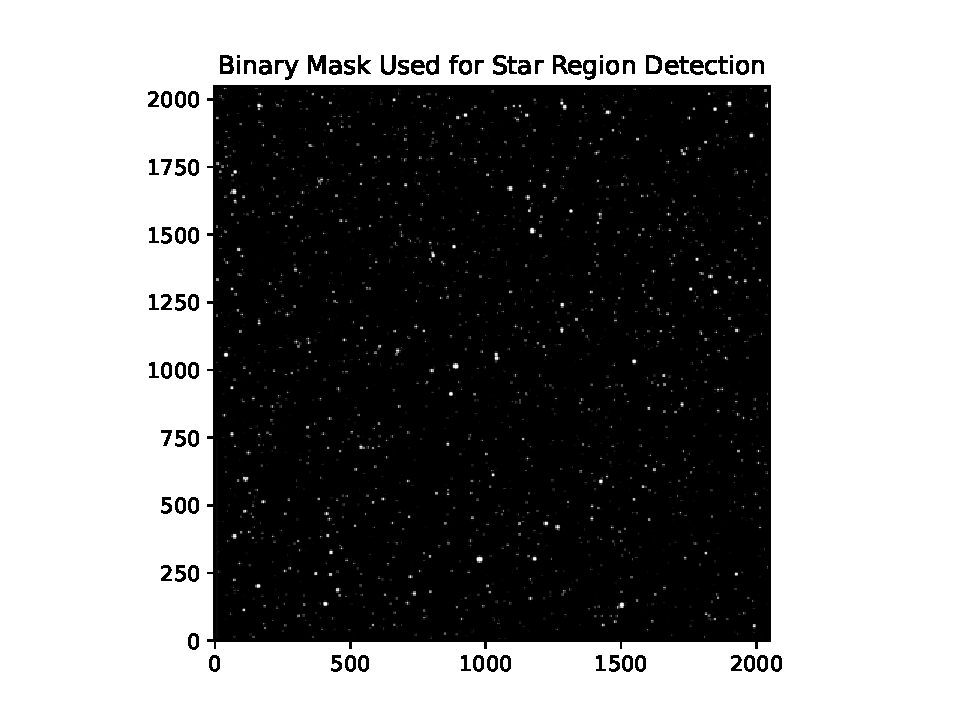
\includegraphics[width=.7\textwidth]{img/binary_mask.pdf}
    \caption{The binary mask of the sky image, with possible regions of stars shown in white.}
    \label{fig:binary}
\end{figure}

Next, \verb|NumPy's| label function is used to assign each of these regions a unique integer. This is done to avoid double counting stars that may get detected as two different stars. Each of these unique integers is looped through, 
and a traditional centroid is calculated for each of the star regions. For each of the centroids, a 2D Gaussian function is also fitted to the same region used for the centroid calculation, using the traditional centroid as the initial guess. An example
of the centroiding process is shown in Figure \ref{fig:centroid}.


\begin{figure}[H]
    \centering
    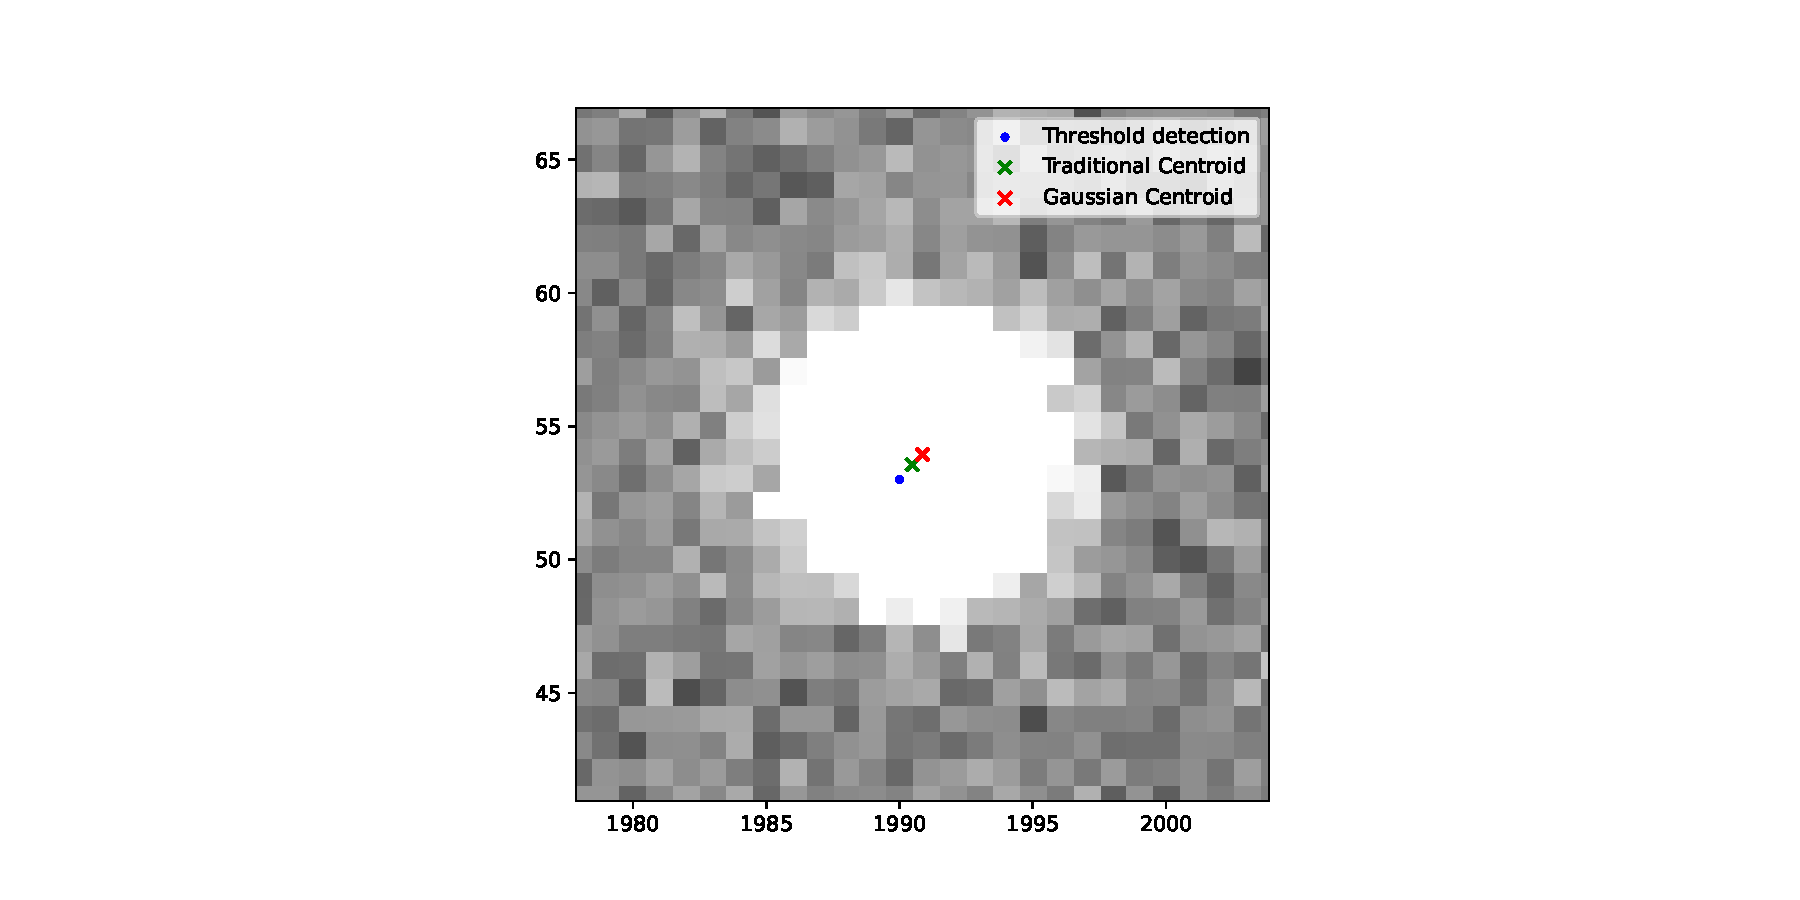
\includegraphics[width=1\textwidth]{img/centroid_0.pdf}
    \caption{An example showing the three-step process used for calculating the pixel coordinates of each star}
    \label{fig:centroid}
\end{figure}

The biggest advantage of using a Gaussian fitting for each of the stars is that it provides a measure of the uncertainty for the centroid. 
The uncertainty is calculated by taking the square root of the diagonal elements of the covariance matrix, and the greatest of these values is used
as the uncertainty for each of the centroids. A threshold uncertainty is set at 0.125, and any star with an uncertainty greater than this value is not 
taken to be the uncertainty for each centroid. This value was set empirically by visual inspection of the centroids, as well as by noticing that the bulk of the centroids fell out of this range. 
For error propagation purposes, the median uncertainty of the distribution of centroid uncertainties is used as the uncertainty for the entire set of centroids. 

\begin{figure}[H]
    \centering
    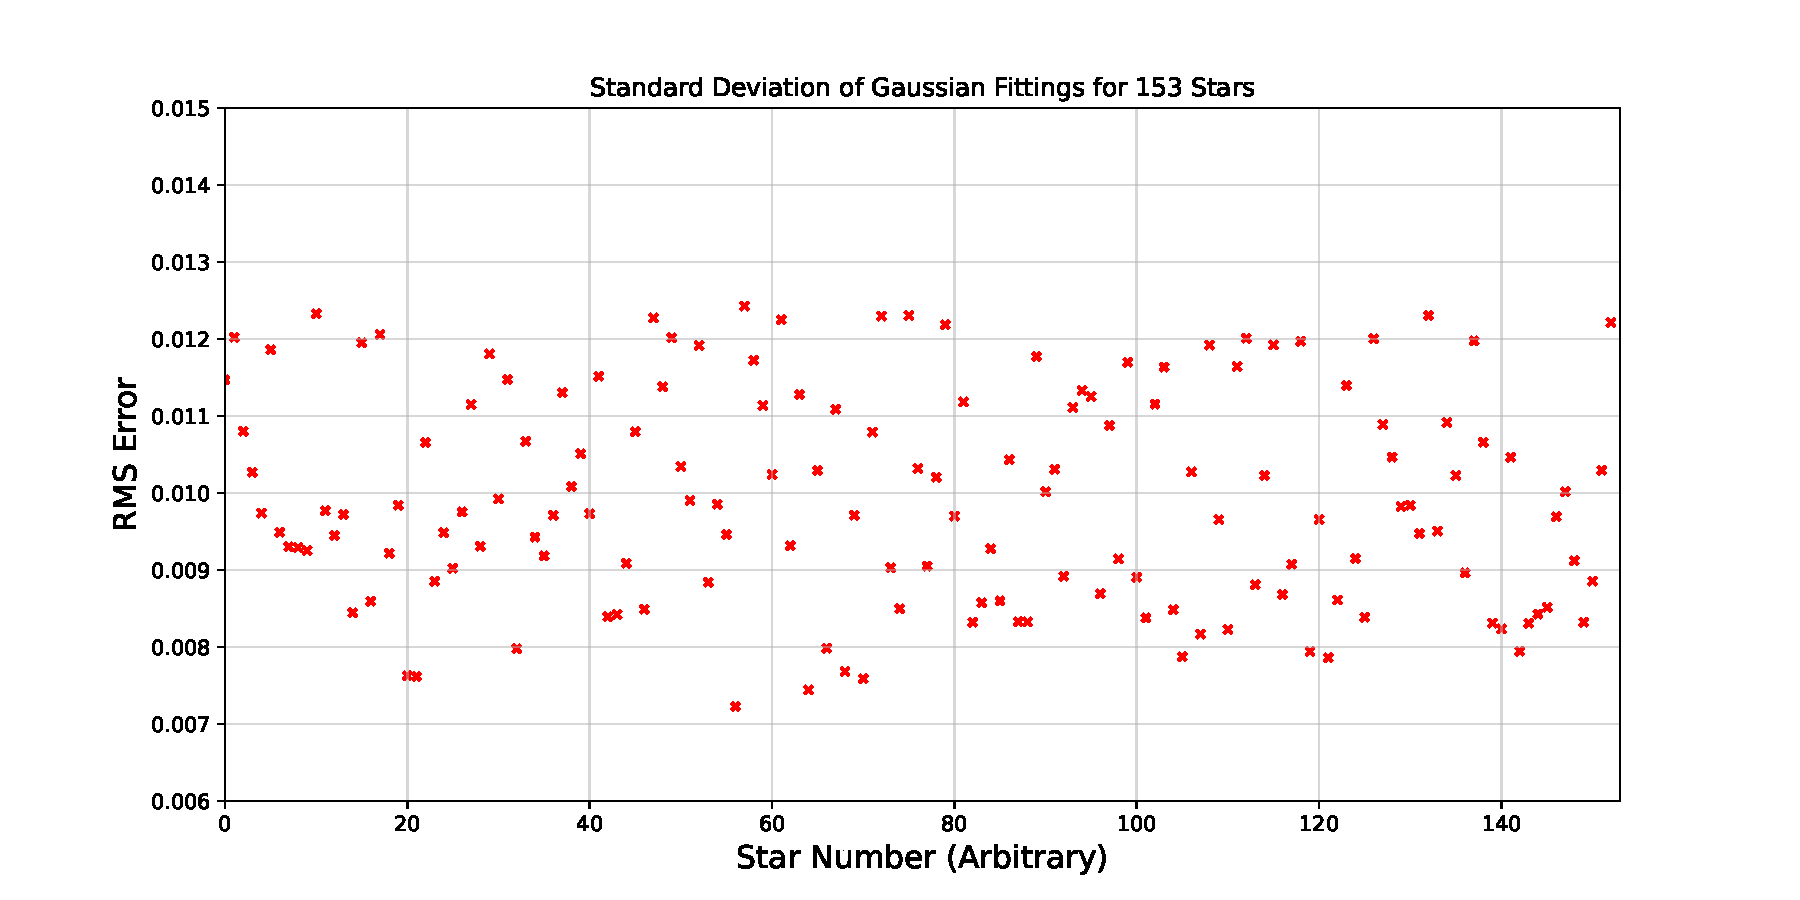
\includegraphics[width=.8\textwidth]{img/centroid_std.pdf}
    \caption{The distribution of uncertainties for the centroids of the stars. The median of this distribution is used as the uncertainty for the entire set of centroids.}
    \label{fig:centroid_std}
\end{figure}

\subsection{Conversion to Standard Coordinates}
After the pixel coordinates of the stars on the CCD are determined, the coordinates of the USNO-B1 stars are converted from celestial coordinates into standard coordinates, and then into approximate pixel positions using the equations 
given in the lab manual. This requires a rotation of 1.2 degrees in the case of this dataset, and a vertical and horizontal translation to account for the difference in origin of the two coordinate systems.

\begin{figure}
    \centering
    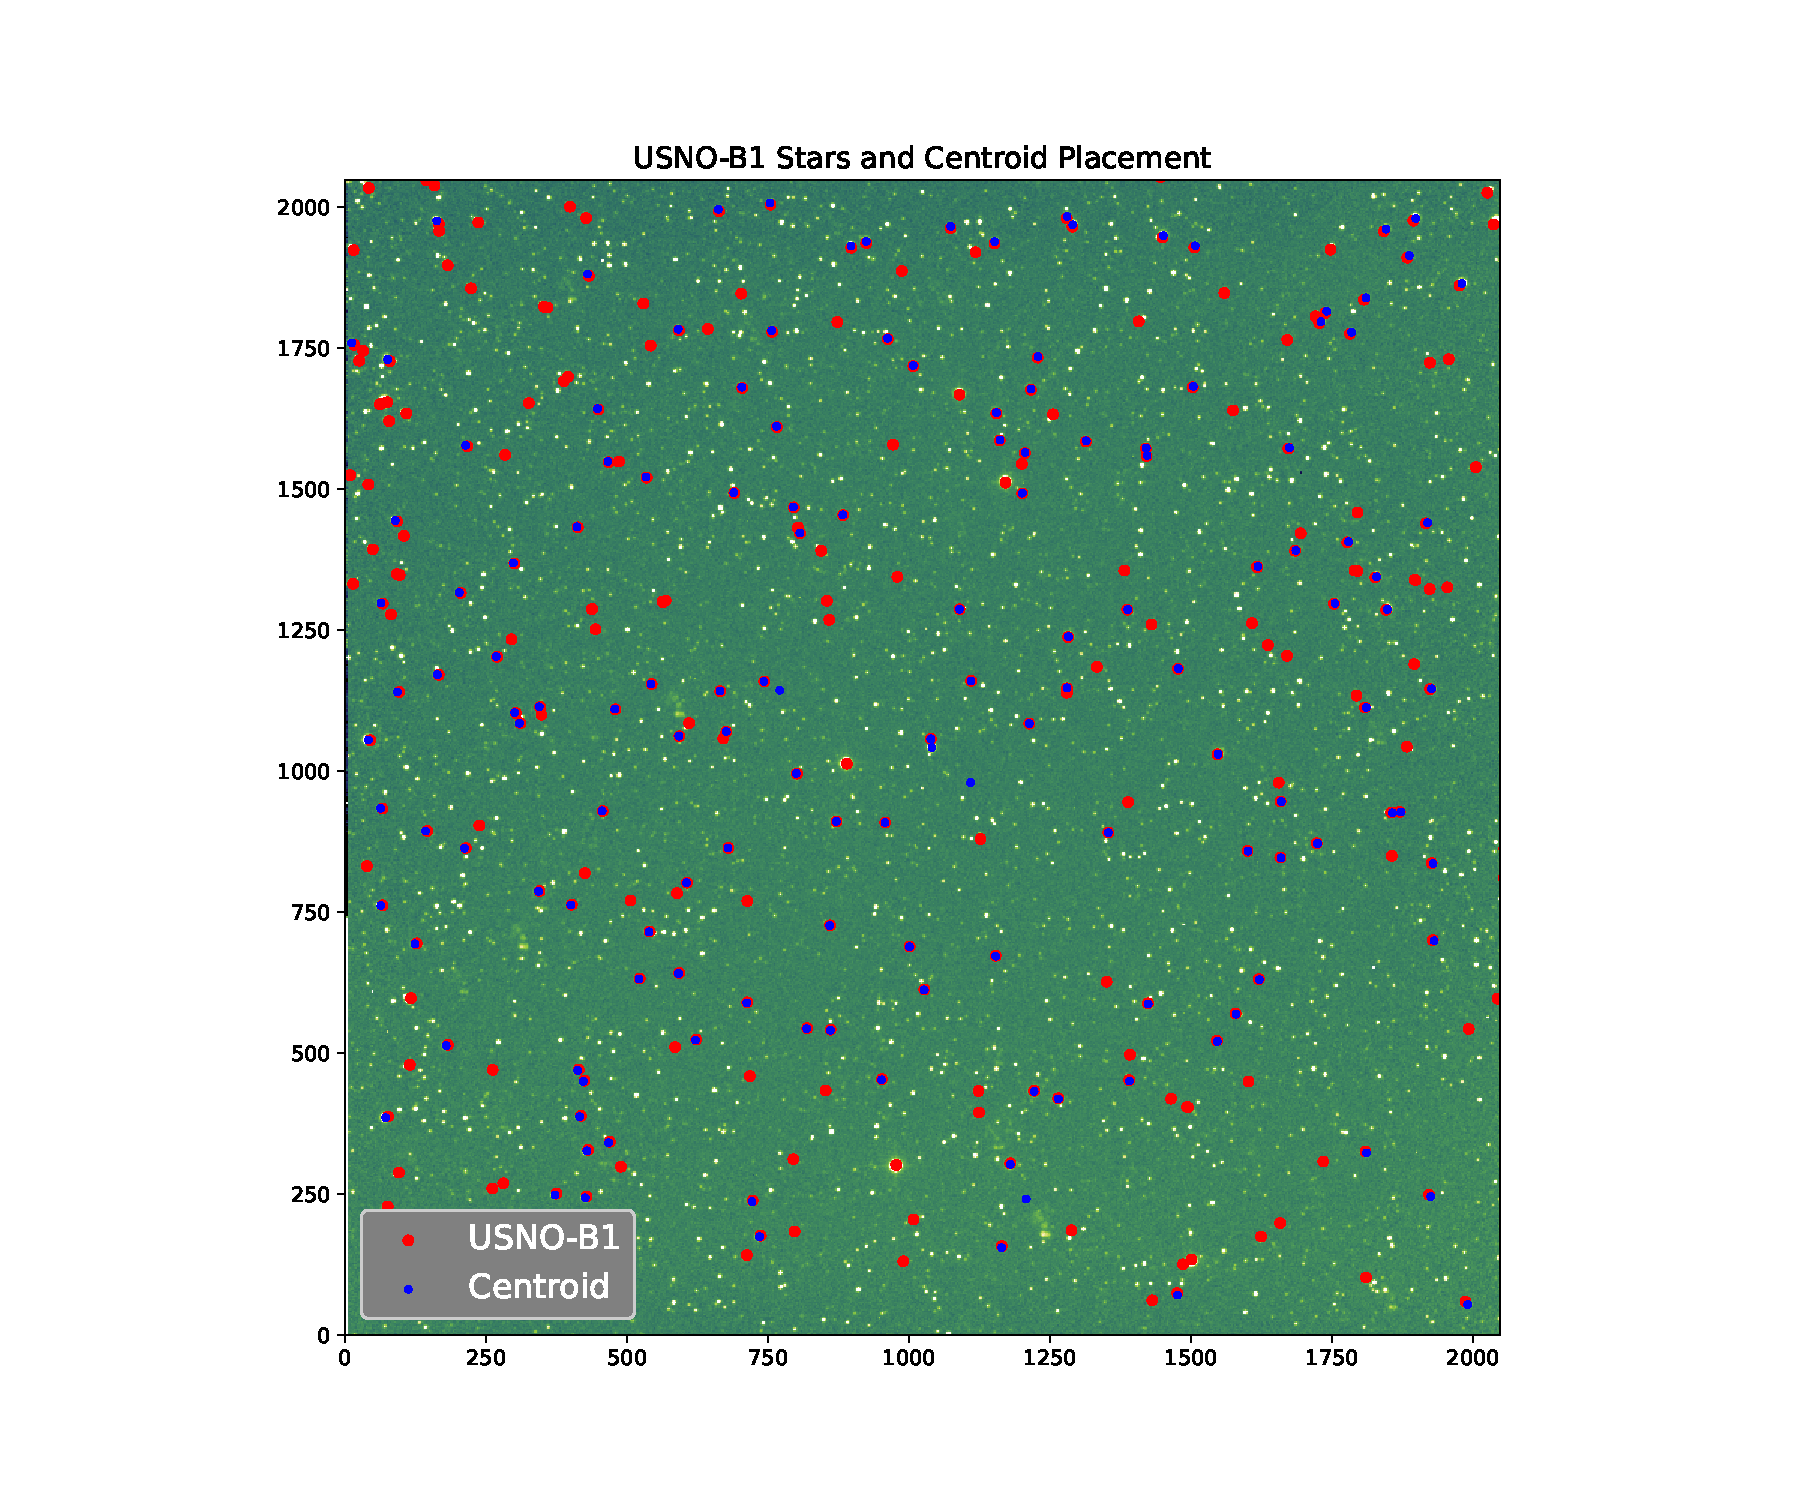
\includegraphics[width=.8\textwidth]{img/standard_coords.pdf}
    \caption{The USNO-B1 star positions converted into approximate pixel positions.}
    \label{fig:approx_coords}
\end{figure}

\subsection{Cross-Matching with the USNO-B1 Catalog}

The euclidean distance is now calculated between each of the centroids and all the other stars in the filtered USNO-B1 catalog, with a 12 pixel threshold 
to be considered as a possible match. The star with the smallest distance is then chosen as the cross-matched star, and the right ascension and declination is associated with the pixel coordinates of the centroid stored in a \verb|Pandas| data frame.
The residuals associated with this initial transformation are shown in Figure \ref{fig:residuals}.

\begin{figure}[H]
    \centering
    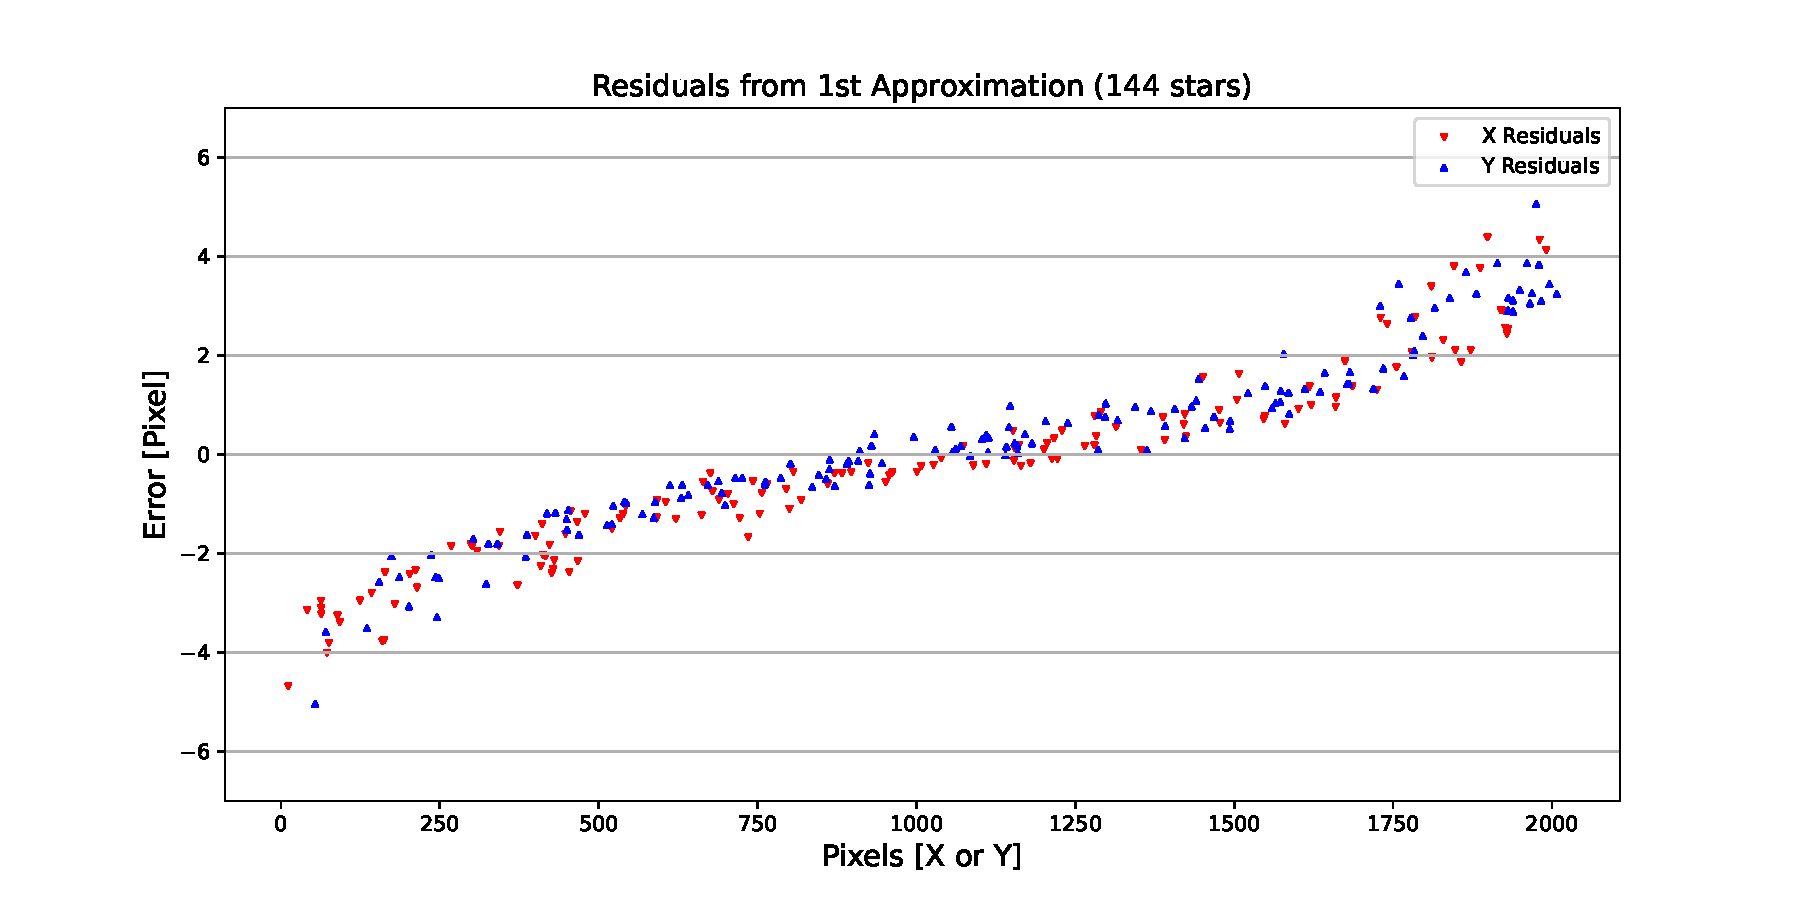
\includegraphics[width=1\textwidth]{img/approx_residuals.pdf}
    \caption{The residuals of the cross-matching between the centroids and the USNO-B1 catalog.}
    \label{fig:residuals}
\end{figure}

\subsection{Plate Solution}

Finally, a linear least squares fitting is applied to find a direct mapping between the standard coordinates of the USNO-B1 stars and the pixel coordinates 
of the centroids. The residuals of this first attempt at a plate solution are shown in Figure \ref{fig:plate_residuals}.

\begin{figure}[H]
    \centering
    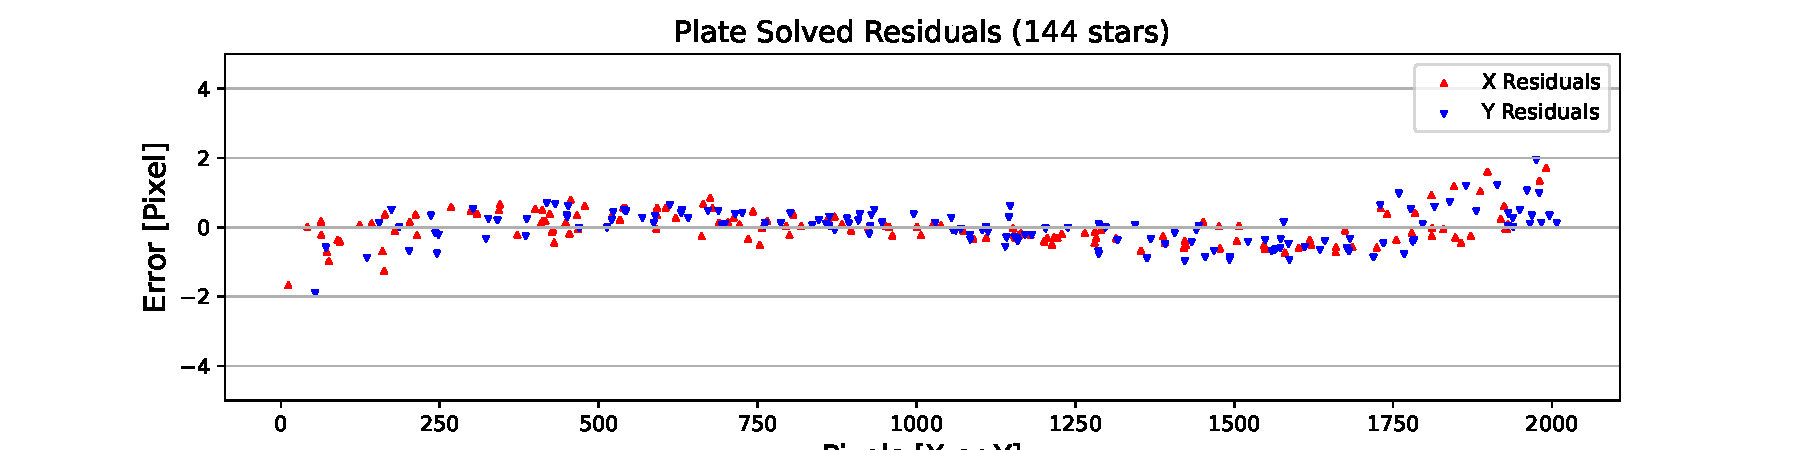
\includegraphics[width=1\textwidth]{img/1stsolve_residuals.pdf}
    \caption{The residuals of the initial plate solution.}
    \label{fig:plate_residuals}
\end{figure}

This initial transformation gave a $\chi^2_{x}$ value of 34.86 and $\chi^2_{y}$ value of 38.93, which is not ideal, but is still acceptable for a first iteration and a great improvement 
over the first approximation. A histogram comparing the initial approximation to the least squares plate solution is shown in Figure \ref{fig:plate_solution}. The vast majority of the points 
are within 1.5 pixels of error.

\begin{figure}[H]
    \centering
    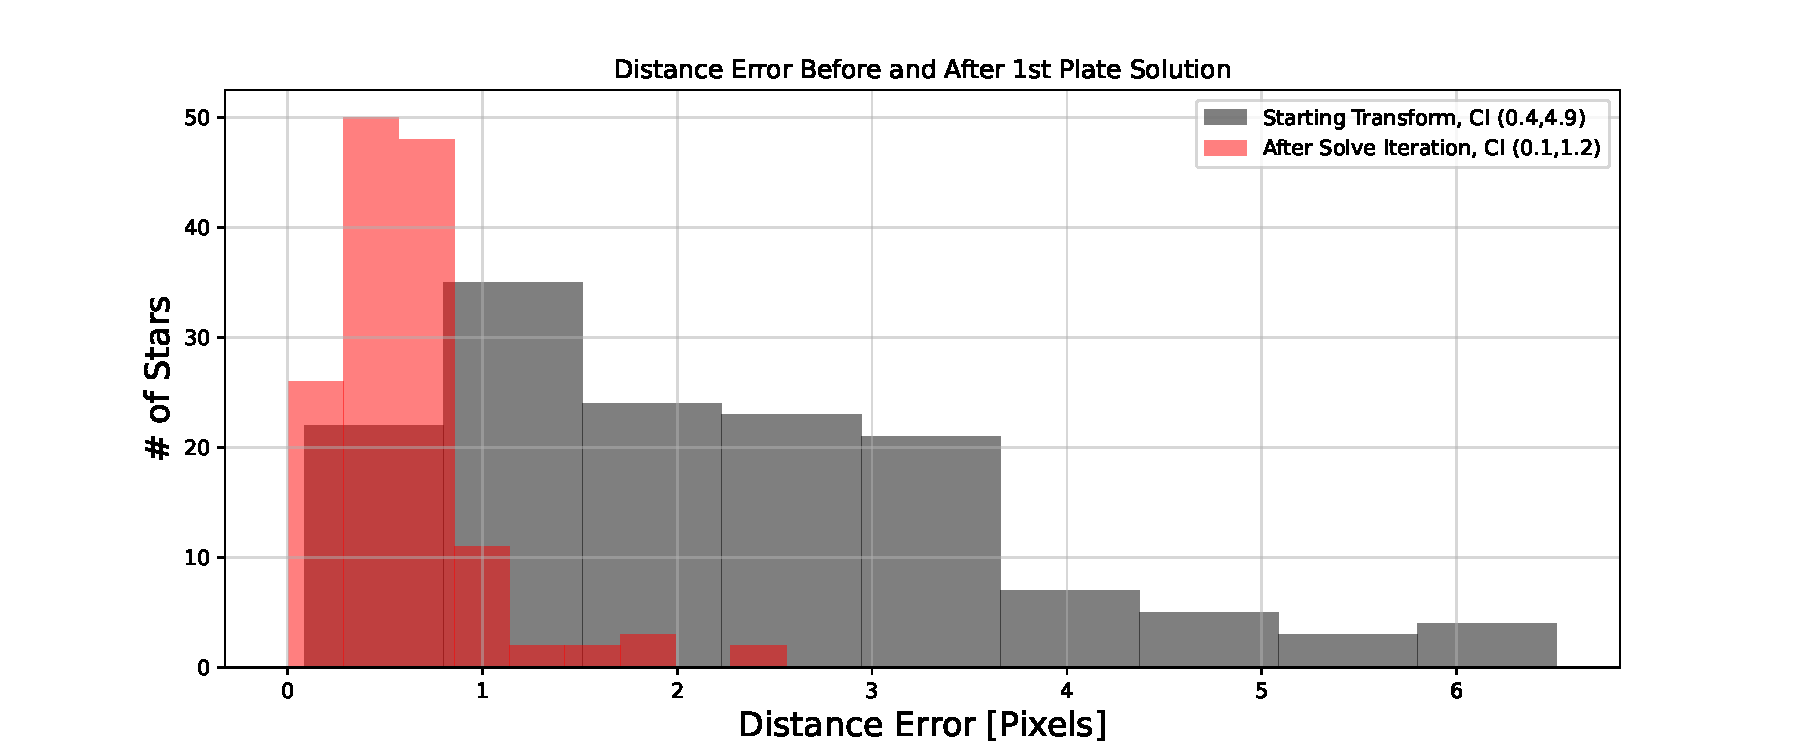
\includegraphics[width=1\textwidth]{img/plate_hist.pdf}
    \caption{A histogram showing the comparison between the initial transformation and the least squares solution. The vast majority of points are 
    within 1.5 pixels error.}
    \label{fig:plate_solution}
\end{figure}

Next, all the points with residuals greater than 1 pixel are removed from the Pandas data frame, and the least squares solver is run again. 
The residuals of this transformation are shown in Figure \ref{fig:plate_residuals2}. Now all the residuals are almost within 1 pixel. 
The $\chi^2_{x}$ value is 18.5, and the $\chi^2_{y}$ value is 18.5. This is still not great, but is pretty good considering the number of sample points used.
The RMS error of this transformation is 0.392, which will be used for error propagation purposes when calculating the velocity of 26 Proserpina.

\begin{figure}[H]
    \centering
    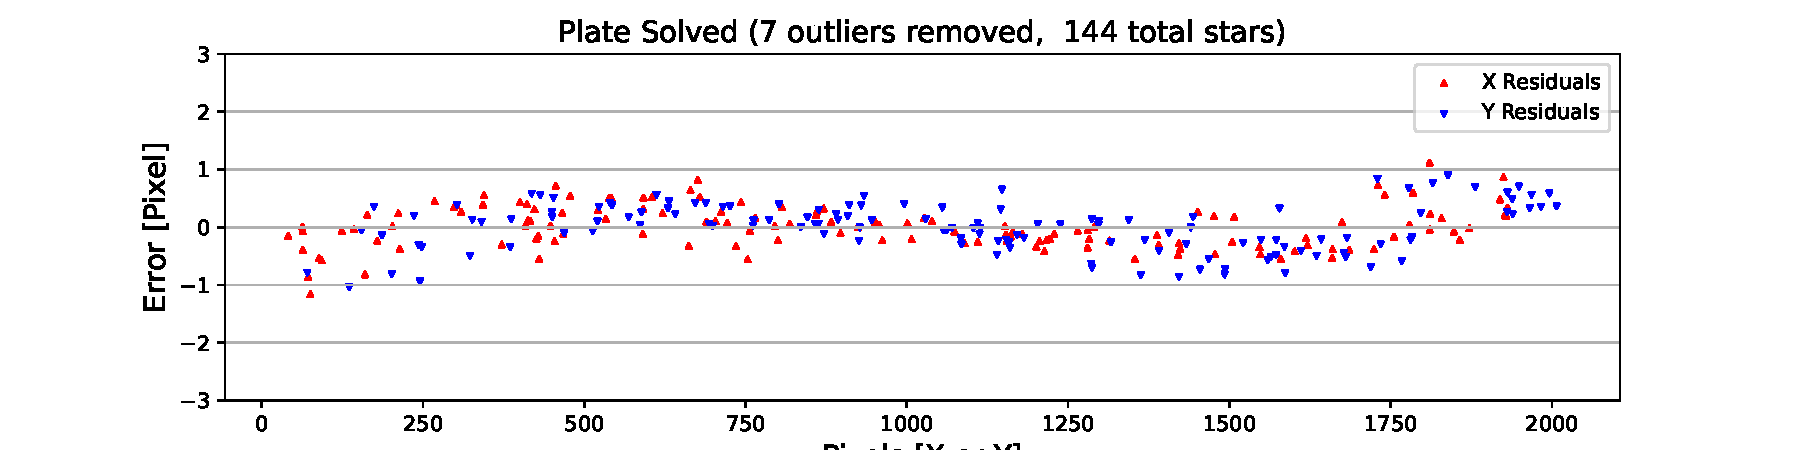
\includegraphics[width=1\textwidth]{img/final_residuals.pdf}
    \caption{The residuals of the plate solution after the second iteration.}
    \label{fig:plate_residuals2}
\end{figure}

\subsection{Locating 26 Proserpina}
Finding the position of 26 Proserpina in each frame is done by first finding the asteroid's approximate celestial coordinates using the NASA JPL Horizons ephemeris system. The plate solution is then 
applied to these approximate coordinates, and the approximate pixel position of the asteroid is found and verified by eye between each frame. These approximate coordinates are not perfect, and the asteroid's 
position is also manually adjusted before the centroid is calculated. The details of this approximation are shown in Table \ref{tab:26pros}. 

\begin{table}[H]
    \centering
    \begin{tabular}{|c|c|c|c|c|c|}
        \hline
        Date & Ephemeris RA & Ephemeris Dec & Approximate Pixel Position & Required Offset from Ephemeris\\
        \hline
        2012-01-20 & 05:24:06.75  &  +26:58:48.3 & (1041, 1040) &  (0,-2) pixels\\
        2012-01-21 & 05:23:33.06 &  +26:58:03.9 & (1045, 999) &  (-10, +5) pixels\\
        2012-01-23 & 05:22:30.16 &  +26:56:32.4 & (1059, 915) &  (-30, +115) pixels\\
        2012-01-26 & 05:21:14.29 &  +26:54:24.8 & (1646,851) &  (-12, +92) pixels\\
        \hline
    \end{tabular}
    \caption{The plate solution applied to JPL Horizons ephemeris coordinates of 26 Proserpina to obtain the approximate pixel position of the asteroid on each
    day.}
    \label{tab:26pros}
\end{table}

Finally, the centroids of 26 Proserpina are calculated in each frame using the same 3-step method used for the background stars. The plate solution's inverse transformation matrix is applied to these coordinates, which gives the asteroid's true position 
in the celestial coordinate system. The results of this process are displayed in table \ref{tab:26pros_centroids} and Figure \ref{fig:pros_cen}.

\begin{table}[H]
    \centering
    \begin{tabular}{|c|c|c|c|c|}
        \hline
        Date & Gaussian Centroid [Pixels] & Uncertainty & Plate Solved (RA, Dec) [Deg] \\
        \hline
        2012-01-20 & (1041.119, 1041.815) & $\pm 0.007$ & (81.0283, 26.980) \\
        2012-01-21 & (1035.49, 1004.28) & $\pm 0.011$ &  (80.891, 26.970) \\
        2012-01-23 & (1030.99, 1029.82) & $\pm 0.011$ & (80.634, 26.977) \\
        2012-01-26 & (1633.90, 944.45) & $\pm 0.013$ & (80.313, 26.395) \\
        \hline
    \end{tabular}
    \caption{The centroid coordinates of 26 Proserpina, and the plate solved celestial coordinates of the asteroid.}
    \label{tab:26pros_centroids}
\end{table}

\begin{figure}[H]
    \centering
    \begin{subfigure}[b]{0.49\textwidth}
        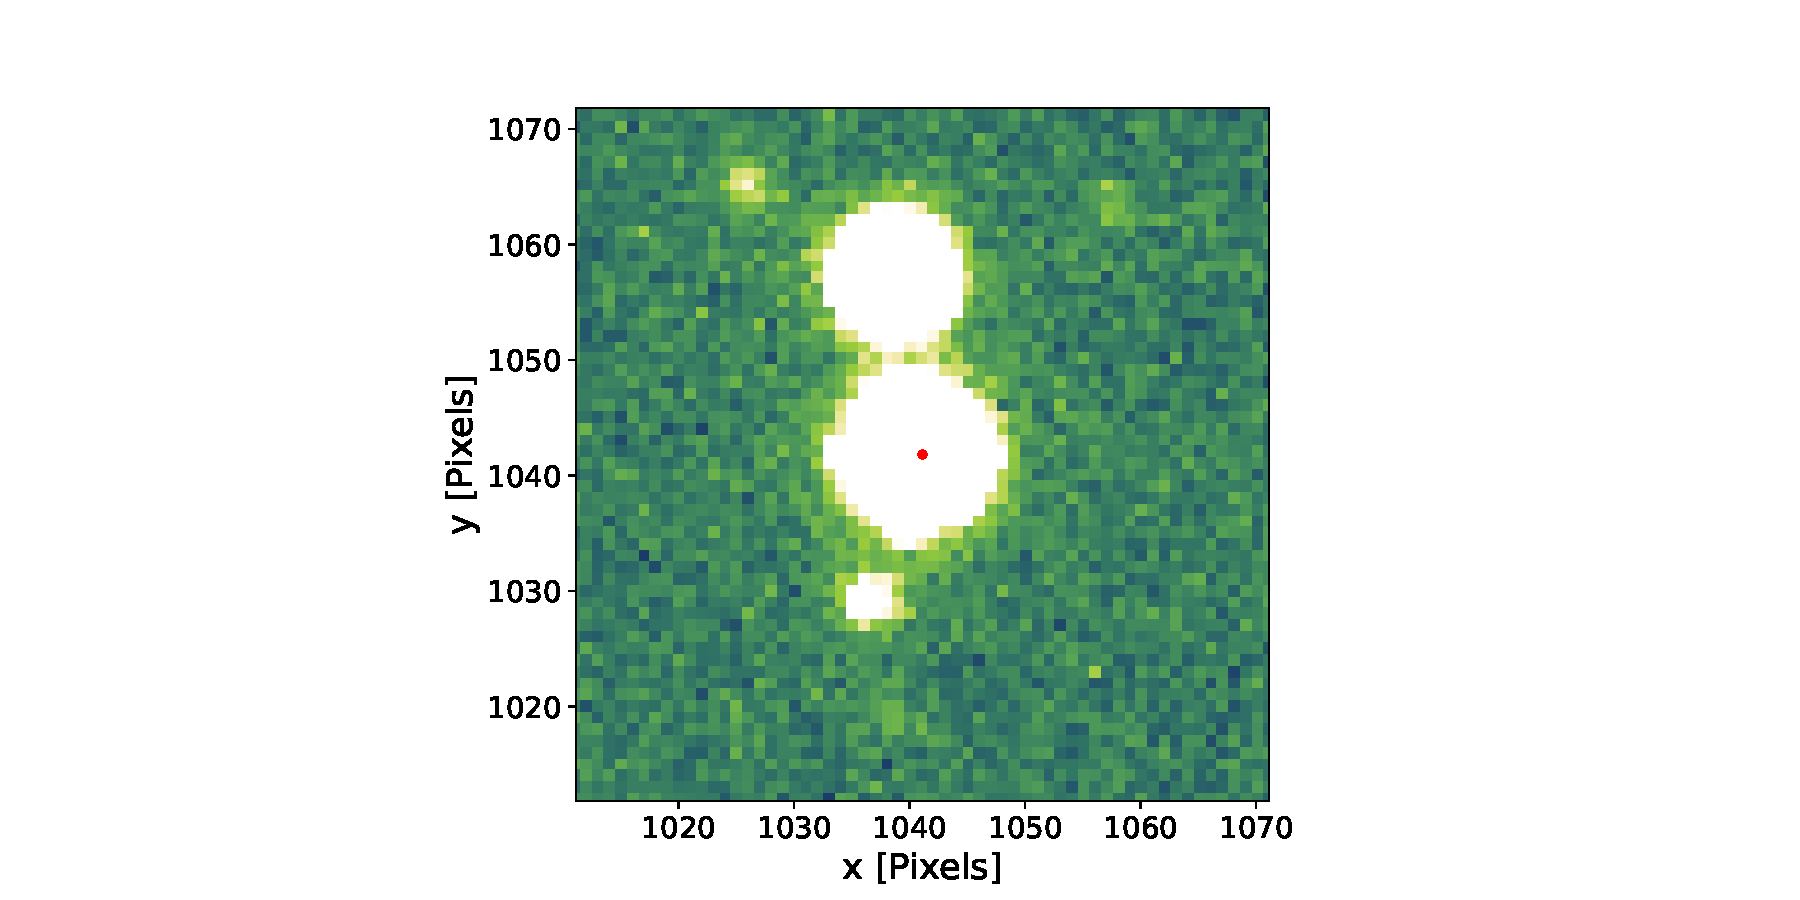
\includegraphics[width=\textwidth]{img/proserpina_day1.pdf}
        \caption{26 Proserpina on 2012-01-20}
        \label{fig:image1}
    \end{subfigure}
    \hfill
    \begin{subfigure}[b]{0.49\textwidth}
        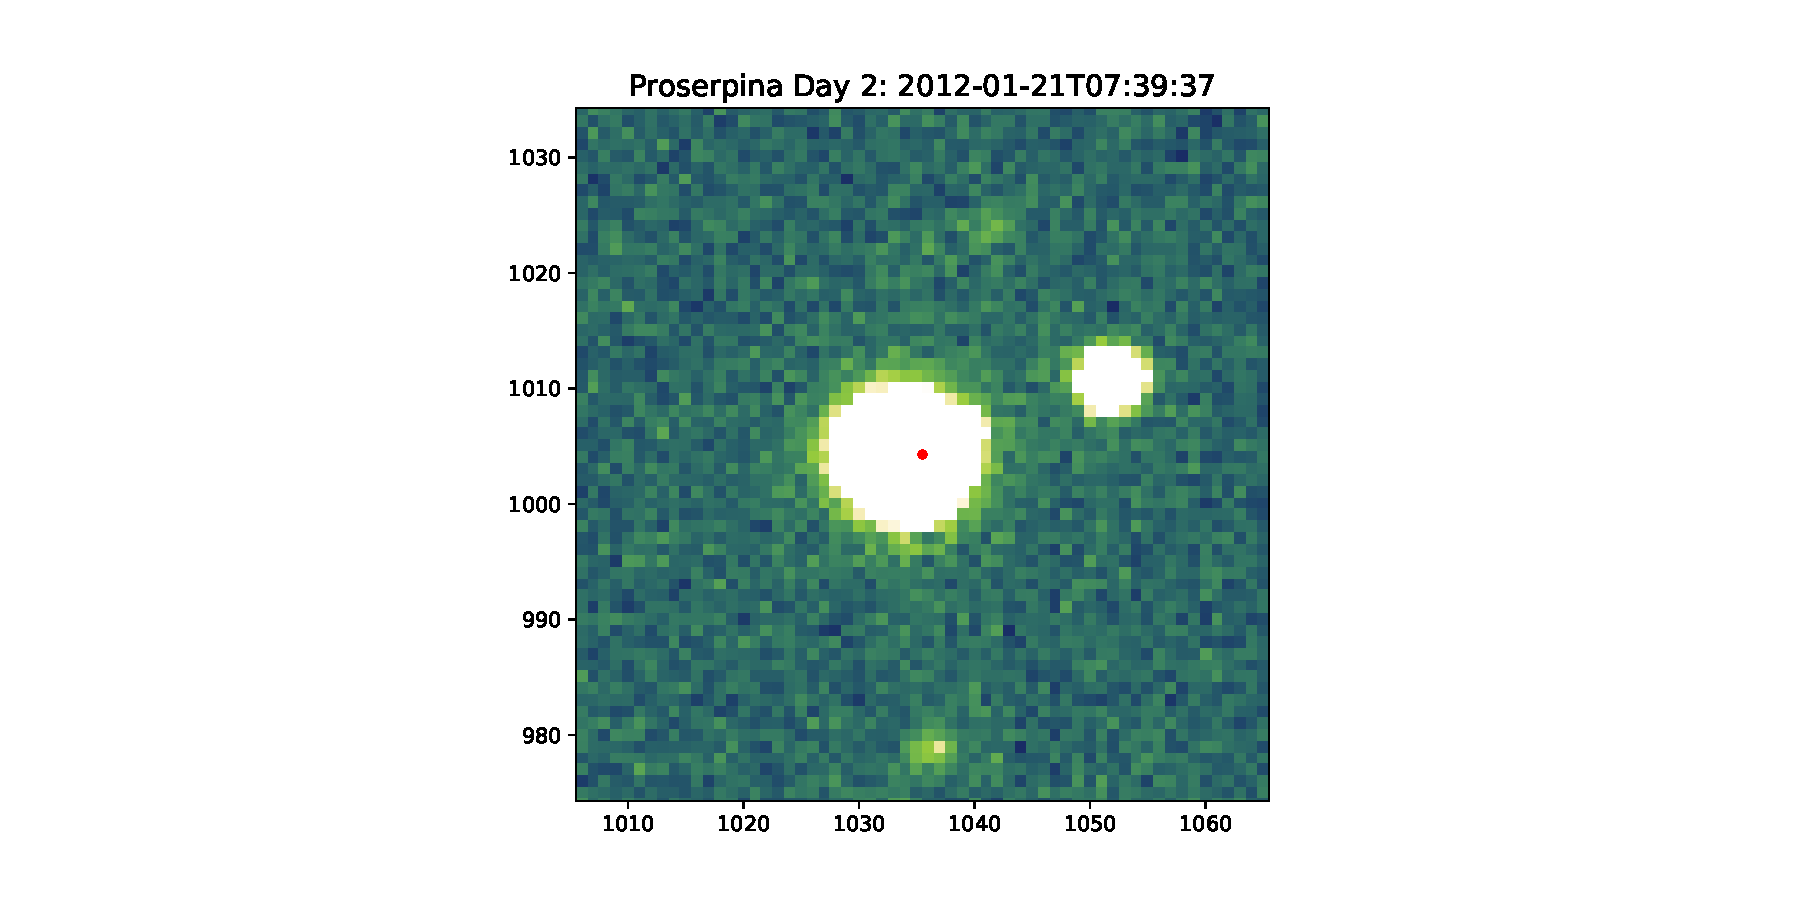
\includegraphics[width=\textwidth]{img/proserpina_day2.pdf}
        \caption{26 Proserpina on 2012-01-21}
        \label{fig:image2}
    \end{subfigure}
    \begin{subfigure}[b]{0.49\textwidth}
        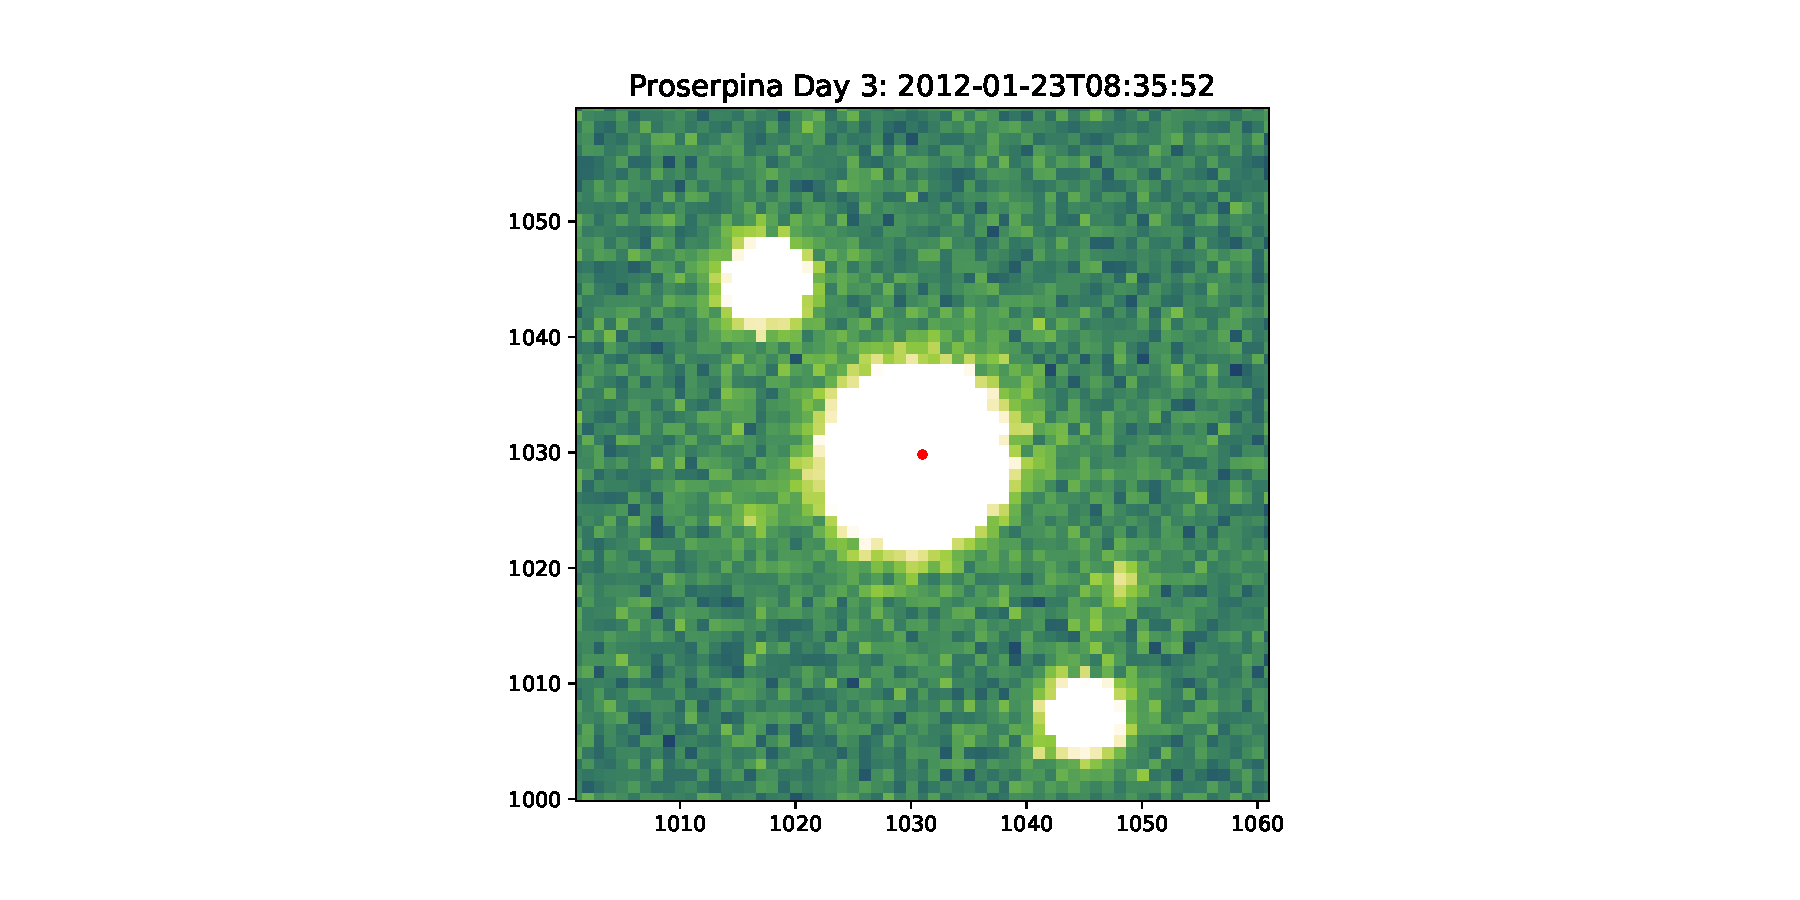
\includegraphics[width=\textwidth]{img/proserpina_day3.pdf}
        \caption{26 Proserpina on 2012-01-23}
        \label{fig:image3}
    \end{subfigure}
    \hfill
    \begin{subfigure}[b]{0.49\textwidth}
        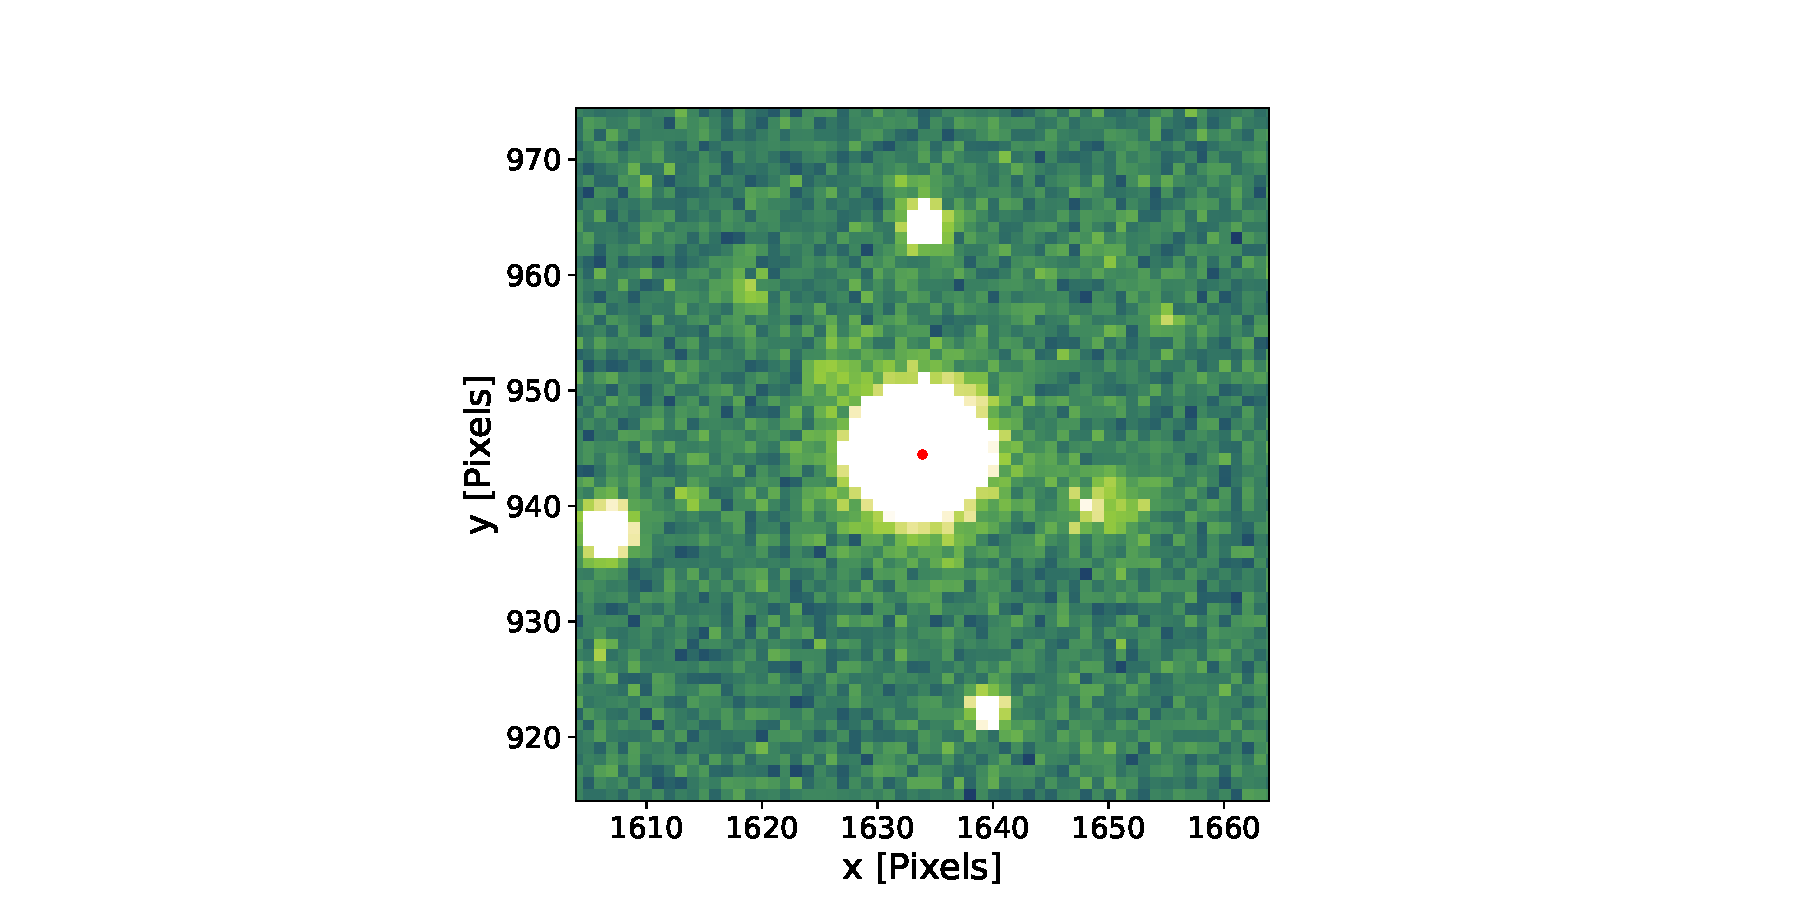
\includegraphics[width=\textwidth]{img/proserpina_day4.pdf}
        \caption{26 Proserpina on 2012-01-26}
        \label{fig:image4}
    \end{subfigure}
    \caption{Centroid Positions of 26 Proserpina on each measurement day.}
    \label{fig:pros_cen}
\end{figure}

\section{Analysis}

\subsection{Proper Motion of 26 Proserpina}

Using the plate solved centroid coordinates of 26 Proserpina, the asteroid's proper motion in the sky can be plotted using celestial coordinates. The pixel position uncertainty
of the asteroid is converted into units of degrees using the nominal pixel scale of the CCD of 0.53 $\frac{arc sec}{pixel}$. These positional errors are of the order of $\approx 10^{-6} \deg$, 
and are deemed to be negligible. The proper motion of 26 Proserpina is shown in Figure \ref{fig:pros_motion}.

\begin{figure}[H]
    \centering
    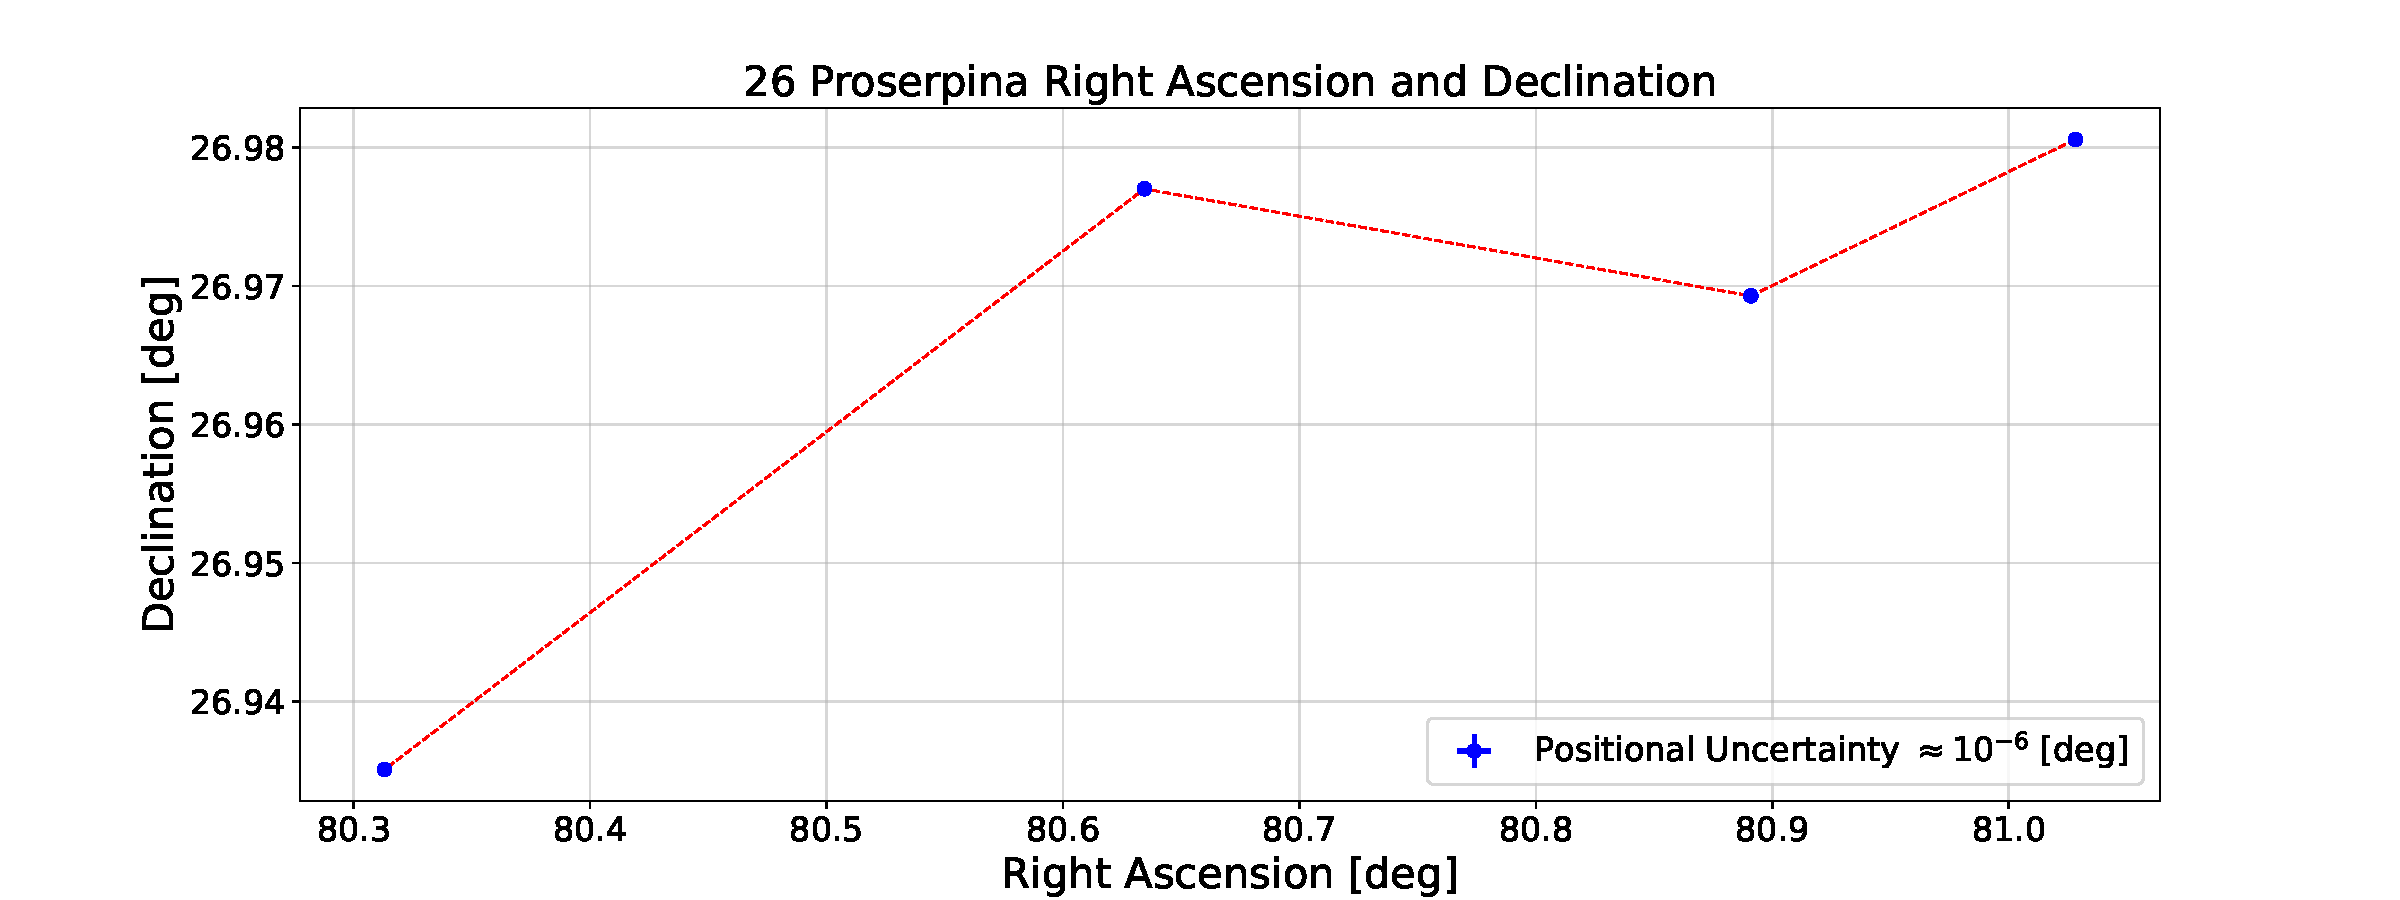
\includegraphics[width=1\textwidth]{img/proserpina_ra_dec.pdf}
    \caption{The proper motion of 26 Proserpina in the sky.}
    \label{fig:pros_motion}
\end{figure}

Since the asteroid's proper motion was measured over the course of 7 Julian days and only 4 measurements, the velocity of the asteroid will have to be determined using 
linear regression. The slope of the best fit line will give the velocities of the asteroid in right ascension and declination, in units of degrees per day. The best fit lines
connecting the 4 measurements over 7 Julian days are shown in Figures \ref{fig:pros_ra} and \ref{fig:pros_dec}.

\begin{figure}[H]
    \centering
    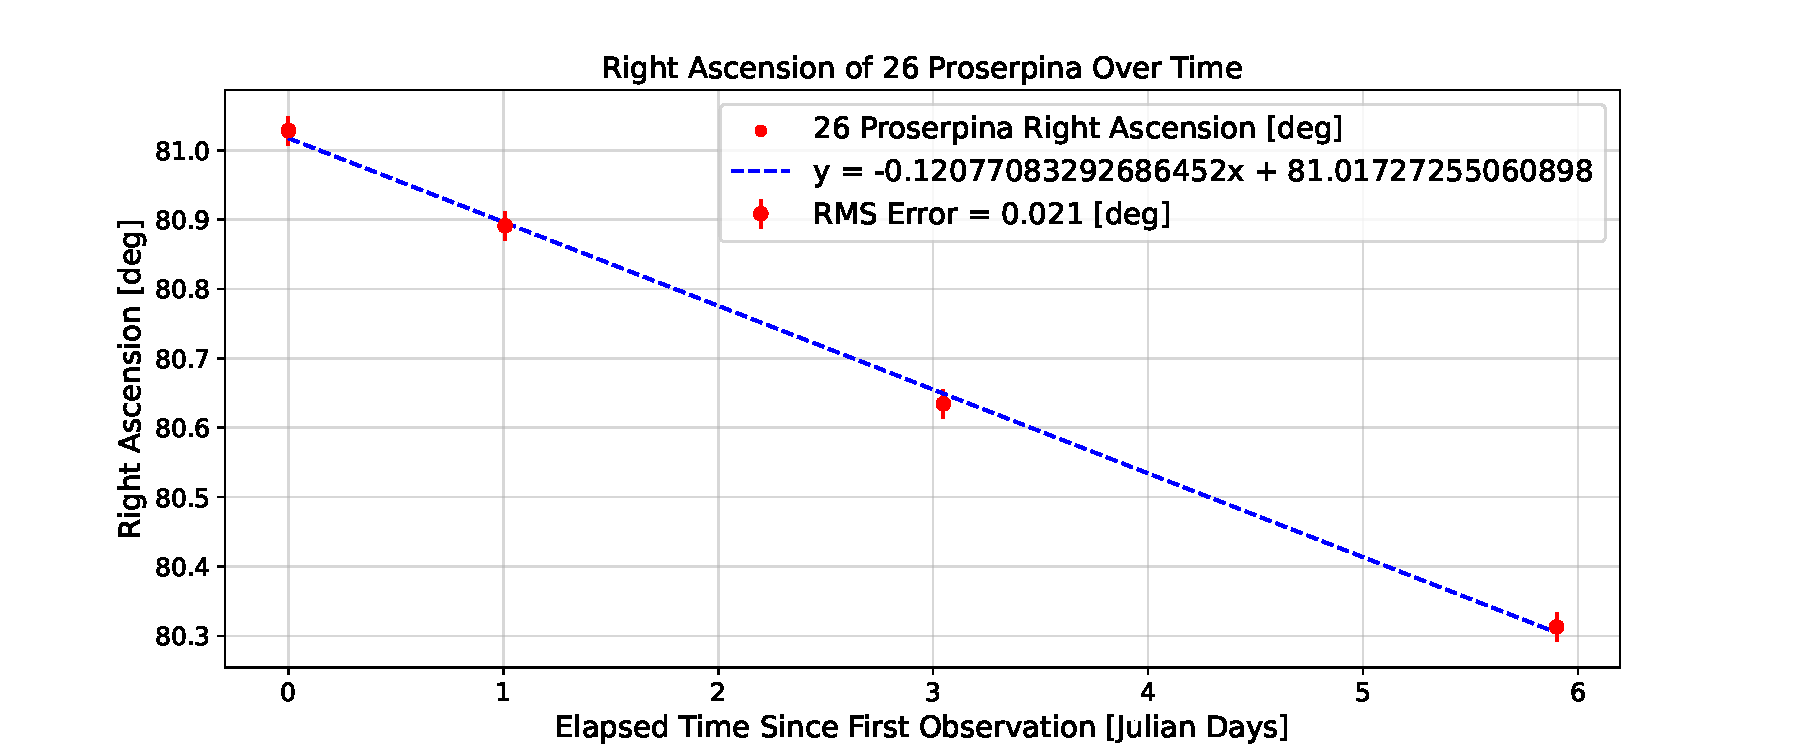
\includegraphics[width=1\textwidth]{img/proserpina_ra_jd.pdf}
    \caption{The proper motion of 26 Proserpina in right ascension, measured in Julian days since the first observation.}
    \label{fig:pros_ra}
\end{figure}

\begin{figure}[H]
    \centering
    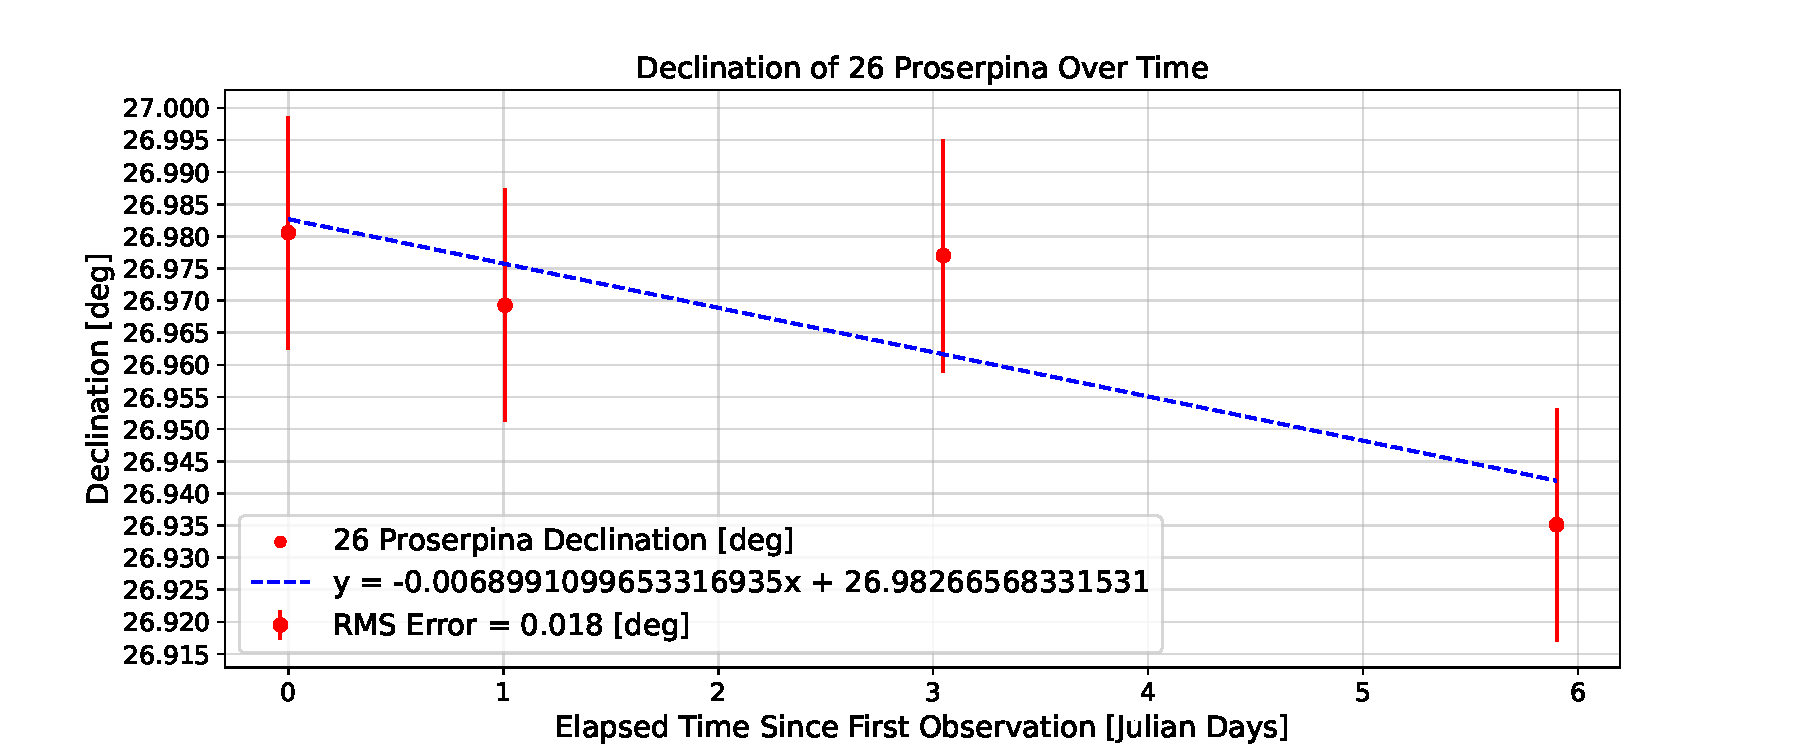
\includegraphics[width=1\textwidth]{img/proserpina_dec_jd.pdf}
    \caption{The proper motion of 26 Proserpina in declination, measured in Julian days since the first observation.}
    \label{fig:pros_dec}
\end{figure}

\subsection{Velocity of 26 Proserpina}

Based on the results of these linear regressions and previously propagated errors, the velocity of 26 Proserpina in right ascension is found to be $-0.30192 \pm 0.052$ arcseconds per hour, 
and the velocity in declination is found to be $-0.01725 \pm 0.045$. By combining these two vector velocities, the magnitude of the asteroid's celestial velocity is found to be $0.30242 \pm 0.069$ 
arc seconds per hour. 

\subsection{Error Propagation}
There are four significant sources of error that can influence the final velocity calculations of 26 Proserpina. The first is the uncertainty in the centroid positions of the stars. Any error in the centroid
placement can lead to stars being matched incorrectly, which can propagate through to the asteroid's position calculations. For error propagation purposes, the total error in these calculations was taken to be the median error
of the uncertainties for each star's Gaussian fitting. For a single star's fitting, the greatest value in the square root of the covariance matrix is taken as the single uncertainty per star. 
The second source of error is the uncertainty in the plate solution, which was characterized by the $\chi^2$ values in the individual axis directions, as well as a final RMS error calculation for the final solution. Accurate positional
measurements of 26 Proserpina are very important as well, and this uncertainty was calculated by the same reasoning as the star centroids. Finally, the uncertainty in the velocity calculations stems from the fact that a linear
regression was used as a basis for the calculation. Considering that the asteroid's position was measured over 7 Julian days, but only 4 measurements were taken, it is likely that the most significant source of error in the calculation stems from this 
final approximation. To simplify calculations, the sources of error are assumed to be independent, and are added in quadrature to obtain the final error in velocity. Any unit conversions necessary were done using the nominal pixel scale given in the lab 
manual. 


\begin{table}[H]
    \hspace{0cm}
    \begin{tabular}{c|c|c|c|c|}
        \hline
        & \textbf{Centroid Star Placement} & \textbf{Plate Solution} & \textbf{Asteroid Centroid Placement} & \textbf{Linear Regression} \\
        \hline
        \textbf{RMS Error} & 0.123 [pixels] & 0.392 [pixels] &  $1.6*10^{-6}$ [pixels] & (0.052, 0.045) [deg] \\
        \hline
    \end{tabular}
    \caption{A detailed summary of where the individual sources of error come from.}
    \label{tab:table_label}
\end{table}

\section{Discussion}
It is clear from the error analysis that the primary source of error comes from the linear regression used to calculate the asteroid's velocity.
The reason that the error is so large is that linear regression is inherently a method of crude approximation for real world data. Four days of measurements are not enough to accurately
determine the slope of best fit, and even a slight change in one of the measurements can propagate to a large change in velocity. Some ways to improve the accuracy of the velocity calculation would be to 
either take more measurements, or to use a more sophisticated method of regression. The linear approximation assumes that the asteroid's velocity is constant over seven days, but realistically this 
is not the case and it varies over time due to the eccentricity of the asteroid's orbit. A more sophisticated method of regression would be to use a polynomial fit, which would determine the velocity of the asteroid
at any given time, but would not be able to give a single value for the velocity like the linear regression provided. 


\begin{appendices}
    
\section{Python Code}
\subsection{Threshold Masking for Star Regions}
\begin{small}
\begin{verbatim}
threshold = 0.0150
stars_x = []
stars_y = []
# Find parts of img where intensity > threshold
binary_img = np.where(science_imgs[0] > threshold, 1, 0)


plt.title("Binary Mask Used for Star Region Detection")
plt.imshow(binary_img, origin='lower', cmap='gray')
plt.savefig("img/binary_mask.pdf")
plt.show()


# Assign each star region a different integer
star_labels, num_stars = label(binary_img)
print(f"Found {num_stars} stars")

# Loop through each region and pick a single point to feed the centroider.
for i in range(1,num_stars+1):
    region_coords = np.where(star_labels == i)
    # Use middle point in each region
    middle_x = np.mean(region_coords[0]).astype(int)
    middle_y = np.mean(region_coords[1]).astype(int) 
    stars_x.append(middle_y)
    stars_y.append(middle_x)
    
size=8
centroid_x, centroid_y, initial_cen_x, initial_cen_y, std = star_gaussian([stars_x, stars_y], 
                                                                          science_imgs[0],threshold,size=size,
                                                                          filter=True)
centroid_catalog = pd.DataFrame({'centroid_x': centroid_x, 'centroid_y': centroid_y})
\end{verbatim}
\end{small}

\subsection{Centroid Finding and Gaussian Fitting}

\begin{small}
\begin{verbatim}
    def star_gaussian(stars, image, threshold, plot=False, size=10, filter=False): 
    uncertainties = []   
    centroids_x_coords = []
    centroids_y_coords = []
    initial_cen_x = []
    initial_cen_y = []
    
    failed_fittings = 0
    size = size
    # 2d gaussian
    def gauss(xy, a, x0, y0, sigma_x, sigma_y, c):
        x, y = xy
        g = a*np.exp(-(x-x0)**2/(2*sigma_x**2) - (y-y0)**2/(2*sigma_y**2)) + c
        return g.ravel()

    for i in range(len(stars[0])):
        box = image[int(stars[1][i])-size:int(stars[1][i])+size, int(stars[0][i])-size:int(stars[0][i])+size]
        
        # Create coordinate matrices and flatten them for fitting
        xx, yy = np.meshgrid(np.arange(box.shape[1]), np.arange(box.shape[0])) 
        xx_flat = xx.ravel()
        yy_flat = yy.ravel()

        # Use centroid equation for initial guess
        x = np.sum(xx * box) / np.sum(box) 
        y = np.sum(yy * box) / np.sum(box) 

        # Fit Gaussian
        if len(yy_flat) != 0:            
            try:
                initial_guess = (1,x,y,size/2,size/2,0)
                popt, pcov = curve_fit(gauss, (xx_flat, yy_flat), box.ravel(), p0=initial_guess, nan_policy='omit')
                if filter:
                    if np.max(np.sqrt(np.diag(pcov))) < 0.0125:
                            
                        # get new centroid
                        centroid_x, centroid_y = popt[1], popt[2]
                        
                        # put the coords back in the original context of the image
                        x = stars[0][i] - size + x
                        y = stars[1][i] - size + y
                        
                        centroid_x = stars[0][i] - size + centroid_x
                        centroid_y = stars[1][i] - size + centroid_y
                        
                        # print(f"Initial Coordinate: {stars[0][i]}, {stars[1][i]}")
                        # print(f"Inital Centroid: {x}, {y}")
                        # print(f"Gaussian Centroid: {centroid_x}, {centroid_y}")
                        
                        # add centroids to list of coords
                        initial_cen_x.append(x)
                        initial_cen_y.append(y)
                        centroids_x_coords.append(centroid_x)
                        centroids_y_coords.append(centroid_y)
                        uncertainties.append(np.max(np.sqrt(np.diag(pcov))))
                                    # get new centroid
                else:
                    centroid_x, centroid_y = popt[1], popt[2]
                    # put the coords back in the original context of the image
                    x = stars[0][i] - size + x
                    y = stars[1][i] - size + y
                    
                    centroid_x = stars[0][i] - size + centroid_x
                    centroid_y = stars[1][i] - size + centroid_y
                    
                    # print(f"Initial Coordinate: {stars[0][i]}, {stars[1][i]}")
                    # print(f"Inital Centroid: {x}, {y}")
                    # print(f"Gaussian Centroid: {centroid_x}, {centroid_y}")
                    
                    # add centroids to list of coords
                    initial_cen_x.append(x)
                    initial_cen_y.append(y)
                    centroids_x_coords.append(centroid_x)
                    centroids_y_coords.append(centroid_y)
                    uncertainties.append(np.max(np.sqrt(np.diag(pcov))))
                
            except RuntimeError:
                failed_fittings += 1
    print(f"Fit {len(centroids_x_coords)} stars")
    print(f"Couldn't fit {failed_fittings} stars")
    return centroids_x_coords, centroids_y_coords, initial_cen_x, initial_cen_y, uncertainties
\end{verbatim}
\end{small}
\subsection{Querying USNO-B1 Catalog and Applying Initial Approximation}

\begin{small}
\begin{verbatim}
    # Get center of field and query USNO-B1
    cof = coord.SkyCoord(header(astroids[0])['RA'], header(astroids[0])['DEC'], unit=(u.hourangle, u.deg), equinox='J2000')
    print(cof.ra.deg, cof.dec.deg)
    fov = 39*u.arcmin
    Vizier.ROW_LIMIT = -1
    usno = Vizier.query_region(cof, width=fov, catalog='USNO-B1')[0].to_pandas()
    
    mag_limit = 14.5
    usno_reduced = usno[usno['R2mag'] < mag_limit].reset_index(drop=True)
    
    fig = plt.figure(figsize=(6, 4)) 
    plt.title("USNO-B1 Stars Used for Plate Solution")      
    plt.scatter(usno_reduced['RAJ2000'], usno_reduced['DEJ2000'], s=2, color='red')
    plt.xlabel('RA (deg)')
    plt.ylabel('Dec (deg)')
    plt.savefig("img/usno.pdf")
    plt.show()
    
    def initial_transform(usno_coords, focal_length, pixel_size, rotation, center_of_field, x_0, y_0):
        alpha = np.deg2rad(usno_coords[:,0])
        delta = np.deg2rad(usno_coords[:,1])
        alpha_0 = center_of_field.ra.rad
        delta_0 = center_of_field.dec.rad
        
        # Project to X and Y
        X = -((np.cos(delta)*np.sin(alpha - alpha_0))/((np.cos(delta_0))*np.cos(delta)*np.cos(alpha-alpha_0)+np.sin(delta)*np.sin(delta_0)))
        Y = -((np.sin(delta_0)*np.cos(delta)*np.cos(alpha-alpha_0)-np.cos(delta_0)*np.sin(delta))/(np.cos(delta_0)*np.cos(delta)*np.cos(alpha-alpha_0)+np.sin(delta)*np.sin(delta_0)))
        
        x_offset = x_0
        y_offset = y_0
    
        
        x = (focal_length/pixel_size)*(X*np.cos(rotation) - Y*np.sin(rotation)) + x_offset
        y = (focal_length/pixel_size)*(X*np.sin(rotation) + Y*np.cos(rotation)) + y_offset
        return x,y
    
    
    pixel_size = 0.009*2
    image_shape = (2048, 2048) # after binning
    #focal_length = 3454 altered empirically for distortion
    focal_length = 3410
    rotation = np.deg2rad(1.2)
    x_offset = 1032
    y_offset = 1042
    usno_stars = np.column_stack((usno_reduced['RAJ2000'], usno_reduced['DEJ2000']))
    
    approximate_x, approximate_y = initial_transform(usno_stars, focal_length, pixel_size, rotation, cof, x_offset, y_offset)
    usno_reduced['approx_x'] = approximate_x
    usno_reduced['approx_y'] = approximate_y
    
    fig = plt.figure(figsize=(12, 10))
    vmin, vmax = ZScaleInterval().get_limits(science_imgs[0])
    plt.imshow(science_imgs[0], cmap='cma:lacerta', origin='lower', vmin=vmin, vmax=vmax)
    plt.scatter(usno_reduced['approx_x'], usno_reduced['approx_y'], marker='.', s=70, color='red', label='USNO-B1')
    plt.title("USNO-B1 Stars and Centroid Placement", fontsize=14)
    plt.scatter(centroid_x, centroid_y, marker='.' , color ='blue', s=30, label='Centroid')
    plt.xlim(0,2048)
    plt.ylim(0,2048)
    plt.legend(loc='lower left', fontsize = 16, labelcolor='white', facecolor='grey', framealpha = 1)
    fig.savefig("img/standard_coords.pdf")
    plt.show()
    
    print("Num centroids" , len(centroid_x))
    print("Num USNO" , len(usno_reduced['approx_x']))
    

\end{verbatim}
\end{small}

\subsection{Cross-Matching with USNO-B1 Catalog}
\begin{small}
\begin{verbatim}
    # Returns nearest star 
    def distance(centroid_catalog, catalog):    # Check distances between each centroid and all stars in catalog
        distances = cdist(centroid_catalog[['centroid_x', 'centroid_y']], catalog[['approx_x', 'approx_y']], metric='euclidean')
        nearest_star_indices = []
        nearest_star_distances = []
        # Find indexes of shortest distances for each centroid
        for i in range(len(distances)):
            nearest_star_indices.append(np.argmin(distances[i]))
            nearest_star_distances.append(np.min(distances[i]))
        return nearest_star_indices, nearest_star_distances
    
    corresponding_usno, min_distance = distance(centroid_catalog, usno_reduced)
    columns = ['USNO-B1.0','RAJ2000','DEJ2000','USNO_approx_x','USNO_approx_y','R2mag','pmRA','pmDE'] 
    distance_threshold = 12
    matched_stars = 0
    total_centroids = len(centroid_catalog)
    for i in range(len(centroid_catalog)):
        if min_distance[i] > distance_threshold:
            usno_reduced.loc[corresponding_usno[i], 'separation'] = np.nan
            usno_reduced.loc[corresponding_usno[i], 'x_centroid'] = centroid_catalog['centroid_x'][i]
            usno_reduced.loc[corresponding_usno[i], 'y_centroid'] = centroid_catalog['centroid_y'][i]
        else:
            usno_reduced.loc[corresponding_usno[i], 'separation'] = min_distance[i]
            usno_reduced.loc[corresponding_usno[i], 'x_centroid'] = centroid_catalog['centroid_x'][i]
            usno_reduced.loc[corresponding_usno[i], 'y_centroid'] = centroid_catalog['centroid_y'][i]
            matched_stars += 1
    print(f"Matched {matched_stars} out of {total_centroids} centroids")
    usno_reduced = usno_reduced[['USNO-B1.0','RAJ2000','DEJ2000','approx_x','approx_y','x_centroid','y_centroid','separation','R2mag','pmRA','pmDE']]
    usno_reduced = usno_reduced.dropna()
\end{verbatim}
\end{small}

\subsection{Plate Solving}
\begin{small}
\begin{verbatim}
alpha = np.deg2rad(usno_reduced['RAJ2000'])
delta = np.deg2rad(usno_reduced['DEJ2000'])
alpha_0 = cof.ra.rad
delta_0 = cof.dec.rad
X = -(np.cos(delta)*np.sin(alpha - alpha_0))/((np.cos(delta_0))*np.cos(delta)*np.cos(alpha-alpha_0)+np.sin(delta)*np.sin(delta_0))
Y = -(np.sin(delta_0)*np.cos(delta)*np.cos(alpha-alpha_0)-np.cos(delta_0)*np.sin(delta))/(np.cos(delta_0)*np.cos(delta)*np.cos(alpha-alpha_0)+np.sin(delta)*np.sin(delta_0))

# Solve for plate constants
f_p = focal_length/pixel_size
a_x = usno_reduced['x_centroid']
a_y = usno_reduced['y_centroid']
col1 = np.array(f_p*X)
col2 = np.array(f_p*Y)
col3 = np.ones_like(col1)
B = np.column_stack((col1, col2, col3))
c_x, uncertainty_x, _,_ = np.linalg.lstsq(B, a_x, rcond=None)
c_y, uncertainty_y,_,_ = np.linalg.lstsq(B, a_y, rcond=None)
T = np.array([[f_p*c_x[0], f_p*c_x[1], c_x[2]], [f_p*c_y[0], f_p*c_y[1], c_y[2]], [0, 0, 1]])

chi_squared_x = uncertainty_x[0] 
chi_squared_y = uncertainty_y[0] 

X_vec = np.array([X,Y,np.ones_like(X)])
x_lstsq = T[0][0]*X + T[0][1]*Y + T[0][2]
y_lstsq = T[1][0]*X + T[1][1]*Y + T[1][2]

print("Chi squared x:",chi_squared_x)
print("Chi squared y:",chi_squared_y)

usno_reduced['x_lstsq'] = x_lstsq
usno_reduced['y_lstsq'] = y_lstsq

plt.title("Plate Solved Positions (1st Iteration)")
plt.scatter(usno_reduced['x_centroid'], usno_reduced['y_centroid'], s=4, color='red', label='Centroids')
plt.scatter(usno_reduced['x_lstsq'], usno_reduced['y_lstsq'], s=4, color='blue', label='Plate Solved Positions')
plt.legend(loc='best')
\end{verbatim}
\end{small}
\subsection{Plotting residuals and other statistical plots}

\begin{small}
\begin{verbatim}

usno_x_approx = np.array(usno_reduced['approx_x'])
usno_y_approx = np.array(usno_reduced['approx_y'])
ccd_x = np.array(usno_reduced['x_centroid'])
ccd_y = np.array(usno_reduced['y_centroid'])
usno_x = np.array(usno_reduced['x_lstsq'])
usno_y = np.array(usno_reduced['y_lstsq'])

def distance(x1,y1,x2,y2):
    return np.sqrt((x1-x2)**2+(y1-y2)**2)

min_dists_before = np.empty_like(usno_x)
min_dists_after = np.empty_like(usno_x)
usno_x_approx = np.array(usno_reduced['approx_x'])

for i in range(usno_x.size):
    min_dists_before[i] = np.min(distance(usno_x_approx[i], usno_y_approx[i], ccd_x, ccd_y))
    min_dists_after[i] = np.min(distance(usno_x[i], usno_y[i], ccd_x, ccd_y))

CI_b = (np.percentile(min_dists_before,5), 
      np.percentile(min_dists_before,95))
CI_a = (np.percentile(min_dists_after,5), 
      np.percentile(min_dists_after,95))

fig = plt.figure(figsize=(12,5))
plt.title("Distance Error Before and After 1st Plate Solution")
plt.hist(min_dists_before, 
         bins = "sturges", 
         color = 'k',
         alpha = 0.5, 
         label=f'Starting Transform, CI ({CI_b[0]:.1f},{CI_b[1]:.1f})')
plt.hist(min_dists_after, 
         bins = "sturges", 
         color = 'r',
         alpha = 0.5, 
         label =f'After Solve Iteration, CI ({CI_a[0]:.1f},{CI_a[1]:.1f})')
plt.grid(alpha=0.5)
plt.xlabel("Distance Error [Pixels]", size = 16)
plt.ylabel("# of Stars", size = 16)
plt.legend()
fig.savefig("img/plate_hist.pdf")
plt.show()

# Plot residuals
fig = plt.figure(figsize=(12,3))
plt.title(f"Residuals from 1st Approximation ({len(usno_reduced)} stars)", fontsize=14)
plt.xlabel("Pixels [X or Y]", fontsize=14)
plt.ylabel("Error [Pixel]", fontsize = 14)
plt.scatter(usno_reduced['x_centroid'], usno_reduced['x_centroid'] - usno_reduced['approx_x'], s=6, color='red', label='X Residuals', marker="v")
plt.scatter(usno_reduced['y_centroid'], usno_reduced['y_centroid'] - usno_reduced['approx_y'], s=6, color='blue', label='Y Residuals', marker="^")
plt.legend(loc='best')
plt.ylim(-7,7)
plt.grid(axis='y')
fig.savefig("img/approx_residuals.pdf")
plt.show()

plt.figure(figsize=(12,3))
plt.title(f"Plate Solved Residuals ({len(usno_reduced)} stars)", fontsize=14)
plt.xlabel("Pixels [X or Y]", fontsize = 14)
plt.ylabel("Error [Pixel]", fontsize = 14)
plt.scatter(usno_reduced['x_centroid'], usno_reduced['x_centroid'] - usno_reduced['x_lstsq'], s=6, color='red', label='X Residuals', marker="^")
plt.scatter(usno_reduced['y_centroid'], usno_reduced['y_centroid'] - usno_reduced['y_lstsq'], s=6, color='blue', label='Y Residuals', marker="v")
plt.ylim(-5,5)
plt.grid(axis='y')
plt.legend(loc='best')
plt.savefig("img/1stsolve_residuals.pdf")

# Add residuals to dataframe
usno_reduced['x_residual'] = usno_reduced['x_centroid'] - usno_reduced['x_lstsq']
usno_reduced['y_residual'] = usno_reduced['y_centroid'] - usno_reduced['y_lstsq']

# Filter final stars by x and y residuals
residual_threshold = 1 # pixels
final_stars = usno_reduced[(np.abs(usno_reduced['x_residual']) < residual_threshold) & (np.abs(usno_reduced['y_residual']) < residual_threshold)]
\end{verbatim}
\end{small}

\subsection{Converting RA Dec to pixels and centroiding 26 Proserpina}
\begin{small}
\begin{verbatim}
    def RADec_pixel(coordinate, center_field):
    alpha = coordinate.ra.rad
    delta = coordinate.dec.rad  
    alpha_0 = center_field.ra.rad
    delta_0 = center_field.dec.rad
    X = -(np.cos(delta)*np.sin(alpha - alpha_0))/((np.cos(delta_0))*np.cos(delta)*np.cos(alpha-alpha_0)+np.sin(delta)*np.sin(delta_0))
    Y = -(np.sin(delta_0)*np.cos(delta)*np.cos(alpha-alpha_0)-np.cos(delta_0)*np.sin(delta))/(np.cos(delta_0)*np.cos(delta)*np.cos(alpha-alpha_0)+np.sin(delta)*np.sin(delta_0))
    x = T[0][0]*X + T[0][1]*Y + T[0][2]
    y = T[1][0]*X + T[1][1]*Y + T[1][2]
    return x, y

# emphemeris = [("81.02", "26.98"), 
#               ("80.88" ,"26.967"), 
#               ("80.62", "26.94"), 
#               ("80.31", "26.907")]


emphemeris = [("05 24 06.75", "26 58 48.3"), 
              ("05 23 33.06" ,"26 58 03.9"), 
              ("05 22 30.16", "26 56 32.4"), 
              ("05 21 14.29", "26 54 24.8")]

coord1 = coord.SkyCoord(emphemeris[0][0], emphemeris[0][1], unit=(u.hourangle, u.deg), equinox='J2000')
coord2 = coord.SkyCoord(emphemeris[1][0], emphemeris[1][1], unit=(u.hourangle, u.deg), equinox='J2000')
coord3 = coord.SkyCoord(emphemeris[2][0], emphemeris[2][1], unit=(u.hourangle, u.deg), equinox='J2000')
coord4 = coord.SkyCoord(emphemeris[3][0], emphemeris[3][1], unit=(u.hourangle, u.deg), equinox='J2000')

# Convert coordinates to pixel space
coord1_cof = coord.SkyCoord(header(astroids[0])['RA'], header(astroids[0])['DEC'], unit=(u.hourangle, u.deg), equinox='J2000')
coord2_cof = coord.SkyCoord(header(astroids[3])['RA'], header(astroids[1])['DEC'], unit=(u.hourangle, u.deg), equinox='J2000')
coord3_cof = coord.SkyCoord(header(astroids[6])['RA'], header(astroids[2])['DEC'], unit=(u.hourangle, u.deg), equinox='J2000')
coord4_cof = coord.SkyCoord(header(astroids[9])['RA'], header(astroids[3])['DEC'], unit=(u.hourangle, u.deg), equinox='J2000')

coord1x, coord1y = RADec_pixel(coord1, coord1_cof)
coord2x, coord2y = RADec_pixel(coord2, coord2_cof)
coord3x, coord3y = RADec_pixel(coord3, coord3_cof)
coord4x, coord4y = RADec_pixel(coord4, coord4_cof)

# Day 1
d1t1 = header(asteroid1[0])['DATE-OBS']
d1t2 = header(asteroid1[1])['DATE-OBS']
d1t3 = header(asteroid1[2])['DATE-OBS']

# Day 2
d2t1 = header(asteroid2[0])['DATE-OBS']
d2t2 = header(asteroid2[1])['DATE-OBS']
d2t3 = header(asteroid2[2])['DATE-OBS']

# Day 3
d3t1 = header(asteroid3[0])['DATE-OBS']
d3t2 = header(asteroid3[1])['DATE-OBS']
d3t3 = header(asteroid3[2])['DATE-OBS']

# Day 4 
d4t1 = header(asteroid4[0])['DATE-OBS']
d4t2 = header(asteroid4[1])['DATE-OBS']
d4t3 = header(asteroid4[2])['DATE-OBS']

timestamps = [d1t1, d1t2, d1t3, d2t1, d2t2, d2t3, d3t1, d3t2, d3t3]

# Centroiding proserpina
box = 10
x1, y1, _, _, d1_uncertainty = star_gaussian([[coord1x],[coord1y-2]], science_imgs[0], plot=True, size=box, threshold = 1, filter = False)
x2, y2, _, _, d2_uncertainty = star_gaussian([[coord2x - 10],[coord2y+5]], science_imgs[3], plot=True, size=box, threshold = 1, filter = False)
x3, y3, _, _, d3_uncertainty = star_gaussian([[coord3x -30],[coord3y + 115]], science_imgs[6], plot=True, size=box, threshold = 1, filter=False)
x4, y4, _, _, d4_uncertainty = star_gaussian([[coord4x -12],[coord4y + 92]], science_imgs[9], plot=True, size=box, threshold = 1, filter=False)

x1, y1 = x1[0], y1[0]
x2, y2 = x2[0], y2[0]
x3, y3 = x3[0], y3[0]
x4, y4 = x4[0], y4[0]

print("Day 1 Uncertainty: ", d1_uncertainty)
print("Day 2 Uncertainty: ", d2_uncertainty)
print("Day 3 Uncertainty: ", d3_uncertainty)
print("Day 4 Uncertainty: ", d4_uncertainty)
pixel_scale = 0.53

uncertainties_arcsec = pixel_scale*np.array([d1_uncertainty, d2_uncertainty, d3_uncertainty, d4_uncertainty])
uncertainties_deg = uncertainties_arcsec/3600
uncertainties_deg = uncertainties_deg.tolist()
uncertainties_deg = [uncertainties[0] for uncertainties in uncertainties_deg]

# x1, y1 = coord1x, coord1y
# x2, y2 = coord2x-10, coord2y+5
# x3, y3 = coord3x - 30, coord3y + 115
# x4, y4 = coord4x-12, coord4y + 92

print(f"Day 1 approx. RA DEC: {coord1.ra.deg, coord1.dec.deg}")
print(f"Day 2 approx. RA DEC: {coord2.ra.deg, coord2.dec.deg}")
print(f"Day 3 approx. RA DEC: {coord3.ra.deg, coord3.dec.deg}")
print(f"Day 4 approx. RA DEC: {coord4.ra.deg, coord4.dec.deg}")

print(f"Day 1 (Px): {coord1x, coord1y}")
print(f"Day 2 (Px): {coord2x, coord2y}")
print(f"Day 3 (Px): {coord3x, coord3y}")
print(f"Day 4 (Px): {coord4x, coord4y}")

x_proserpina = np.array([[x1, x2, x3, x4], [y1, y2, y3, y4], np.ones_like([x1, x2, x3, x4])])

print(f'Day 1 centroid: {x1, y1}')
print(f'Day 2 centroid: {x2, y2}')
print(f'Day 3 centroid: {x3, y3}')
print(f'Day 4 centroid: {x4, y4}')

vmin, max = ZScaleInterval().get_limits(science_imgs[0])

# Day 1 
fig = plt.figure(figsize=(12, 6))
plt.imshow(science_imgs[0], cmap='cma:lacerta', vmin=vmin, vmax=max)
plt.scatter(x1, y1, marker='.', color='red', s=50, label='Centroid 1')
plt.xticks(fontsize=14)
plt.xlim(x1-box-20, x1+box+20)
plt.ylim(y1-box-20, y1+box+20)
plt.yticks(fontsize=14)
plt.xticks(fontsize=14)
plt.xlabel("x [Pixels]", fontsize=17)
plt.ylabel("y [Pixels]", fontsize=17)
fig.savefig("img/proserpina_day1.pdf")
plt.show()

# Day 2
fig = plt.figure(figsize=(12, 6))
plt.imshow(science_imgs[3], cmap='cma:lacerta', origin='lower', vmin=vmin, vmax=max)
plt.scatter(x2, y2, marker='.', color='red', s=50, label='Centroid 2')
plt.xlim(x2-box-20, x2+box+20)
plt.ylim(y2-box-20, y2+box+20)
plt.xticks(fontsize=14)
plt.yticks(fontsize=14)
plt.xlabel("x [Pixels]", fontsize=17)
plt.ylabel("y [Pixels]", fontsize=17)
fig.savefig("img/proserpina_day2.pdf")
plt.show()

# Day 3
fig = plt.figure(figsize=(12, 6))
plt.imshow(science_imgs[6], cmap='cma:lacerta', origin='lower', vmin=vmin, vmax=max)
plt.scatter(x3, y3, marker='.', color='red', s=50, label='Centroid 3')
plt.xlim(x3-box-20, x3+box+20)
plt.ylim(y3-box-20, y3+box+20)
plt.yticks(fontsize=14)
plt.xticks(fontsize=14)
plt.xlabel("x [Pixels]", fontsize=17)
plt.ylabel("y [Pixels]", fontsize=17)
fig.savefig("img/proserpina_day3.pdf")
plt.show()

# Day 4
fig = plt.figure(figsize=(12, 6))
plt.imshow(science_imgs[9], cmap='cma:lacerta', origin='lower', vmin=vmin, vmax=max)
plt.scatter(x4, y4, marker='.', color='red', s=50, label='Centroid 4')
plt.xlim(x4-box-20, x4+box+20)
plt.ylim(y4-box-20, y4+box+20)
plt.yticks(fontsize=14)
plt.xticks(fontsize=14)
plt.xlabel("x [Pixels]", fontsize=17)
plt.ylabel("y [Pixels]", fontsize=17)
fig.savefig("img/proserpina_day4.pdf")
plt.show()

\end{verbatim}
\end{small}

\subsection{Proper Motion and Velocity Calculations / Error Propagation}
\begin{small}
\begin{verbatim}

# Convert to RA and DEC
X_vec_proserpina = np.linalg.inv(T) @ x_proserpina
print(X_vec_proserpina)

X_proserpina = X_vec_proserpina[0]
Y_proserpina = X_vec_proserpina[1]

ra1_proserpina = np.arctan((-X_proserpina[0])/(np.cos(coord1_cof.dec.rad) - Y_proserpina[0]*np.sin(coord1_cof.dec.rad))) + coord1_cof.ra.rad
dec1_proserpina = np.arcsin((np.sin(coord1_cof.dec.rad)+Y_proserpina[0]*np.cos(coord1_cof.dec.rad))/(np.sqrt(1+X_proserpina[0]**2 + Y_proserpina[0]**2)))

ra2_proserpina = np.arctan((-X_proserpina[1])/(np.cos(coord2_cof.dec.rad) - Y_proserpina[1]*np.sin(coord2_cof.dec.rad))) + coord2_cof.ra.rad
dec2_proserpina = np.arcsin((np.sin(coord2_cof.dec.rad) + Y_proserpina[1]*np.cos(coord2_cof.dec.rad))/(np.sqrt(1+X_proserpina[1]**2 + Y_proserpina[1]**2)))

ra3_proserpina = np.arctan((-X_proserpina[2])/(np.cos(coord3_cof.dec.rad) - Y_proserpina[2]*np.sin(coord3_cof.dec.rad))) + coord3_cof.ra.rad
dec3_proserpina = np.arcsin((np.sin(coord3_cof.dec.rad) + Y_proserpina[2]*np.cos(coord3_cof.dec.rad))/(np.sqrt(1+X_proserpina[2]**2 + Y_proserpina[2]**2)))

ra4_proserpina = np.arctan((-X_proserpina[3])/(np.cos(coord4_cof.dec.rad) - Y_proserpina[3]*np.sin(coord4_cof.dec.rad))) + coord4_cof.ra.rad
dec4_proserpina = np.arcsin((np.sin(coord4_cof.dec.rad) + Y_proserpina[3]*np.cos(coord4_cof.dec.rad))/(np.sqrt(1+X_proserpina[3]**2 + Y_proserpina[3]**2)))

proserpina1 = coord.SkyCoord(ra1_proserpina, dec1_proserpina, unit=(u.rad, u.rad), equinox='J2000')
proserpina2 = coord.SkyCoord(ra2_proserpina, dec2_proserpina, unit=(u.rad, u.rad), equinox='J2000')
proserpina3 = coord.SkyCoord(ra3_proserpina, dec3_proserpina, unit=(u.rad, u.rad), equinox='J2000')
proserpina4 = coord.SkyCoord(ra4_proserpina, dec4_proserpina, unit=(u.rad, u.rad), equinox='J2000')

proserpina_calculated_ra = [proserpina1.ra.deg, proserpina2.ra.deg, proserpina3.ra.deg, proserpina4.ra.deg]
proserpina_calculated_dec = [proserpina1.dec.deg, proserpina2.dec.deg, proserpina3.dec.deg, proserpina4.dec.deg]

print(f"Day 1 approx RA DEC (deg): , {coord1.ra.deg, coord1.dec.deg}")
print(f"Day 1 Calculated RA DEC (deg): {proserpina1.ra.deg, proserpina1.dec.deg}")
print(f"Day 2 approx RA DEC (deg): , {coord2.ra.deg, coord2.dec.deg}")
print(f"Day 2 Calculated RA DEC (deg): {proserpina2.ra.deg, proserpina2.dec.deg}")
print(f"Day 3 approx RA DEC (deg): , {coord3.ra.deg, coord3.dec.deg}")
print(f"Day 3 Calculated RA DEC (deg): {proserpina3.ra.deg, proserpina3.dec.deg}")
print(f"Day 4 approx RA DEC (deg): , {coord4.ra.deg, coord4.dec.deg}")
print(f"Day 4 Calculated RA DEC (deg): {proserpina4.ra.deg, proserpina4.dec.deg}")

ast_cen_median_uncertainty = np.median(uncertainties_deg)
print("median asteroid uncertainty centroid: ", ast_cen_median_uncertainty)

fig = plt.figure(figsize=(16, 6))
plt.title("26 Proserpina Right Ascension and Declination", fontsize=20)
plt.xlabel("Right Ascension [deg]", fontsize=20)
plt.ylabel("Declination [deg]", fontsize=20)
plt.xticks(fontsize=16)
plt.yticks(fontsize=16)
plt.errorbar(proserpina_calculated_ra, proserpina_calculated_dec, xerr=uncertainties_deg, yerr=uncertainties_deg,lw=2, fmt='o', color='blue', label=r"Positional Uncertainty $\approx 10^{-6}$ [deg]")
#plt.scatter(proserpina_calculated_ra, proserpina_calculated_dec, s=10, color='red', label="26 Proserpina Position")
plt.plot(proserpina_calculated_ra, proserpina_calculated_dec, color='red', linestyle='--', linewidth=1)
plt.grid(alpha=0.5)
plt.legend(loc="lower right", fontsize=16)
plt.savefig("img/proserpina_ra_dec.pdf")
plt.show()

from astropy.time import Time
dates = [d1t1, d2t1, d3t1, d4t1]
times_dt = [Time(date).datetime for date in dates]
times_jd = [Time(date).jd for date in dates]
normalized_times_jd = times_jd - times_jd[0]

# Fit a line to the data 
coefficients_ra, residuals_ra, _, _, _ = np.polyfit(normalized_times_jd, proserpina_calculated_ra, 1, full=True)
coefficients_dec, residuals_dec, _, _, _ = np.polyfit(normalized_times_jd, proserpina_calculated_dec, 1, full=True)

ra_line = np.poly1d(coefficients_ra)
dec_line = np.poly1d(coefficients_dec)
ra_rms = np.sqrt(residuals_ra/len(residuals_ra))
dec_rms = np.sqrt(residuals_dec/len(residuals_dec))

fig = plt.figure(figsize=(12, 5))
plt.title("Right Ascension of 26 Proserpina Over Time", fontsize=14)
plt.xlabel("Elapsed Time Since First Observation [Julian Days]", fontsize=14)
plt.ylabel("Right Ascension [deg]", fontsize=14)
plt.scatter(normalized_times_jd, proserpina_calculated_ra, s=20, color='red', label="26 Proserpina Right Ascension [deg]")
plt.errorbar(normalized_times_jd, proserpina_calculated_ra, yerr=ra_rms, fmt='o', color='red', label=f"RMS Error = {np.round(ra_rms, 3)[0]} [deg]")
plt.plot(normalized_times_jd, ra_line(normalized_times_jd), color='blue', label = f"y = {coefficients_ra[0]}x + {coefficients_ra[1]}", ls='--')
plt.grid(alpha=0.5)
plt.legend(fontsize=14)
plt.xticks(fontsize=12)
plt.yticks(fontsize=12)
plt.savefig("img/proserpina_ra_jd.pdf")
plt.show()

fig = plt.figure(figsize=(12, 5))
plt.yticks(np.arange(26.9,27, 0.005))
plt.title("Declination of 26 Proserpina Over Time", fontsize=14)
plt.xlabel("Elapsed Time Since First Observation [Julian Days]", fontsize=14)
plt.ylabel("Declination [deg]", fontsize=14)
plt.scatter(normalized_times_jd, proserpina_calculated_dec, s=20, color='red', label="26 Proserpina Declination [deg]")
plt.errorbar(normalized_times_jd, proserpina_calculated_dec, yerr=dec_rms, fmt='o', color='red', label=f"RMS Error = {np.round(dec_rms, 3)[0]} [deg]")
plt.plot(normalized_times_jd, dec_line(normalized_times_jd), color='blue', label=f"y = {coefficients_dec[0]}x + {coefficients_dec[1]}", ls='--')
plt.legend(loc = 'lower left', fontsize=14)
plt.grid(alpha=0.5)
plt.xticks(fontsize=12)
plt.yticks(fontsize=12)
fig.savefig("img/proserpina_dec_jd.pdf")
plt.show()

# Convert deg to arcsec / minute
ra_rms = (ra_rms*3600)/1440 # arcseconds per minute
dec_rms = (dec_rms*3600)/1440 # arcseconds per minute

print("RA RMS: ", ra_rms)
print("RA Residuals: ", residuals_ra)
print("DEC RMS: ", dec_rms)
print("DEC Residuals: ", residuals_dec)

print("Velocity in RA (deg/day): ", coefficients_ra[0])
print("Velocity in DEC (deg/day): ", coefficients_dec[0])

print("Velocity in RA (arcsec/min): ", (coefficients_ra[0]*3600)/(1440))
print("Velocity in DEC (arcsec/min): ", (coefficients_dec[0]*3600)/(1440))
print("Celestial Velocity Magnitude (arcsec/min): ", np.sqrt((coefficients_ra[0]*3600/1440)**2 + (coefficients_dec[0]*3600/1440)**2))

############### Sources of Error ####################
pixel_scale = 0.53 # arcsec/pixel
print("---- Error Propagation ----")
rmse_stars = np.sqrt(np.sum(std)**2/len(std))
print("RMSE Stars (pixel): ",rmse_stars)
print("RMSE Plate (pixel): ",rmse_fit)
rmse_stars_arcsec = pixel_scale*rmse_stars # arcsec
rmse_plate_arcsec = pixel_scale*rmse_fit # arcsec
rmse_stars_arces_min = rmse_stars_arcsec/10080
rmse_plate_arcsec_min = rmse_plate_arcsec/10080
print("RMS Stars (arcsec): ", rmse_stars_arcsec)
print("RMS Plate (arcsec): ", rmse_plate_arcsec)

# Ast centroid
median_astroid_rms_cen_per_min = (pixel_scale*ast_cen_median_uncertainty)/10080

# linear regression 
print("RMS Asteroid (RA) (arcsec/min): ", ra_rms)
print("RMS Asteroid (DEC) (arcsec/min): ", dec_rms)
print("-----")
print("Final propogated error for RA velocity (arcsec/min): ", np.sqrt(rmse_stars_arces_min**2 + median_astroid_rms_cen_per_min**2 + rmse_plate_arcsec_min**2 + ra_rms**2))
print("Final propogated error for DEC velocity (arcsec/min): ", np.sqrt(rmse_stars_arces_min**2 + median_astroid_rms_cen_per_min**2 + rmse_plate_arcsec_min**2 + dec_rms**2))
print("Final propogated error for velocity magnitude (arcsec/min): ", np.sqrt(rmse_stars_arces_min**2 + median_astroid_rms_cen_per_min**2 + rmse_plate_arcsec_min**2 + ra_rms**2 + dec_rms**2))
\end{verbatim}
\end{small}

\end{appendices}


\end{document}